\documentclass[1p]{elsarticle_modified}
%\bibliographystyle{elsarticle-num}

%\usepackage[colorlinks]{hyperref}
%\usepackage{abbrmath_seonhwa} %\Abb, \Ascr, \Acal ,\Abf, \Afrak
\usepackage{amsfonts}
\usepackage{amssymb}
\usepackage{amsmath}
\usepackage{amsthm}
\usepackage{scalefnt}
\usepackage{amsbsy}
\usepackage{kotex}
\usepackage{caption}
\usepackage{subfig}
\usepackage{color}
\usepackage{graphicx}
\usepackage{xcolor} %% white, black, red, green, blue, cyan, magenta, yellow
\usepackage{float}
\usepackage{setspace}
\usepackage{hyperref}

\usepackage{tikz}
\usetikzlibrary{arrows}

\usepackage{multirow}
\usepackage{array} % fixed length table
\usepackage{hhline}

%%%%%%%%%%%%%%%%%%%%%
\makeatletter
\renewcommand*\env@matrix[1][\arraystretch]{%
	\edef\arraystretch{#1}%
	\hskip -\arraycolsep
	\let\@ifnextchar\new@ifnextchar
	\array{*\c@MaxMatrixCols c}}
\makeatother %https://tex.stackexchange.com/questions/14071/how-can-i-increase-the-line-spacing-in-a-matrix
%%%%%%%%%%%%%%%

\usepackage[normalem]{ulem}

\newcommand{\msout}[1]{\ifmmode\text{\sout{\ensuremath{#1}}}\else\sout{#1}\fi}
%SOURCE: \msout is \stkout macro in https://tex.stackexchange.com/questions/20609/strikeout-in-math-mode

\newcommand{\cancel}[1]{
	\ifmmode
	{\color{red}\msout{#1}}
	\else
	{\color{red}\sout{#1}}
	\fi
}

\newcommand{\add}[1]{
	{\color{blue}\uwave{#1}}
}

\newcommand{\replace}[2]{
	\ifmmode
	{\color{red}\msout{#1}}{\color{blue}\uwave{#2}}
	\else
	{\color{red}\sout{#1}}{\color{blue}\uwave{#2}}
	\fi
}

\newcommand{\Sol}{\mathcal{S}} %segment
\newcommand{\D}{D} %diagram
\newcommand{\A}{\mathcal{A}} %arc


%%%%%%%%%%%%%%%%%%%%%%%%%%%%%5 test

\def\sl{\operatorname{\textup{SL}}(2,\Cbb)}
\def\psl{\operatorname{\textup{PSL}}(2,\Cbb)}
\def\quan{\mkern 1mu \triangleright \mkern 1mu}

\theoremstyle{definition}
\newtheorem{thm}{Theorem}[section]
\newtheorem{prop}[thm]{Proposition}
\newtheorem{lem}[thm]{Lemma}
\newtheorem{ques}[thm]{Question}
\newtheorem{cor}[thm]{Corollary}
\newtheorem{defn}[thm]{Definition}
\newtheorem{exam}[thm]{Example}
\newtheorem{rmk}[thm]{Remark}
\newtheorem{alg}[thm]{Algorithm}

\newcommand{\I}{\sqrt{-1}}
\begin{document}

%\begin{frontmatter}
%
%\title{Boundary parabolic representations of knots up to 8 crossings}
%
%%% Group authors per affiliation:
%\author{Yunhi Cho} 
%\address{Department of Mathematics, University of Seoul, Seoul, Korea}
%\ead{yhcho@uos.ac.kr}
%
%
%\author{Seonhwa Kim} %\fnref{s_kim}}
%\address{Center for Geometry and Physics, Institute for Basic Science, Pohang, 37673, Korea}
%\ead{ryeona17@ibs.re.kr}
%
%\author{Hyuk Kim}
%\address{Department of Mathematical Sciences, Seoul National University, Seoul 08826, Korea}
%\ead{hyukkim@snu.ac.kr}
%
%\author{Seokbeom Yoon}
%\address{Department of Mathematical Sciences, Seoul National University, Seoul, 08826,  Korea}
%\ead{sbyoon15@snu.ac.kr}
%
%\begin{abstract}
%We find all boundary parabolic representation of knots up to 8 crossings.
%
%\end{abstract}
%\begin{keyword}
%    \MSC[2010] 57M25 
%\end{keyword}
%
%\end{frontmatter}

%\linenumbers
%\tableofcontents
%
\newcommand\colored[1]{\textcolor{white}{\rule[-0.35ex]{0.8em}{1.4ex}}\kern-0.8em\color{red} #1}%
%\newcommand\colored[1]{\textcolor{white}{ #1}\kern-2.17ex	\textcolor{white}{ #1}\kern-1.81ex	\textcolor{white}{ #1}\kern-2.15ex\color{red}#1	}

{\Large $\underline{12a_{0327}~(K12a_{0327})}$}

\setlength{\tabcolsep}{10pt}
\renewcommand{\arraystretch}{1.6}
\vspace{1cm}\begin{tabular}{m{100pt}>{\centering\arraybackslash}m{274pt}}
\multirow{5}{120pt}{
	\centering
	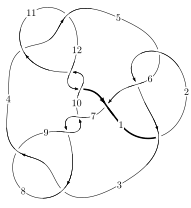
\includegraphics[width=112pt]{../../../GIT/diagram.site/Diagrams/png/1128_12a_0327.png}\\
\ \ \ A knot diagram\footnotemark}&
\allowdisplaybreaks
\textbf{Linearized knot diagam} \\
\cline{2-2}
 &
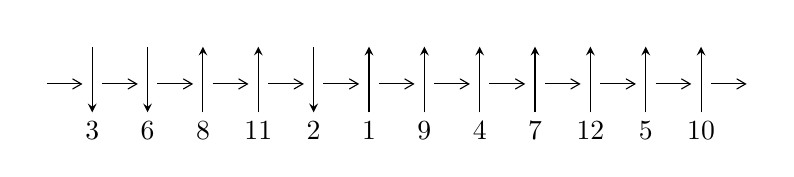
\begin{tikzpicture}[x=20pt, y=17pt]
	% nodes
	\node (C0) at (0, 0) {};
	\node (C1) at (1, 0) {};
	\node (C1U) at (1, +1) {};
	\node (C1D) at (1, -1) {3};

	\node (C2) at (2, 0) {};
	\node (C2U) at (2, +1) {};
	\node (C2D) at (2, -1) {6};

	\node (C3) at (3, 0) {};
	\node (C3U) at (3, +1) {};
	\node (C3D) at (3, -1) {8};

	\node (C4) at (4, 0) {};
	\node (C4U) at (4, +1) {};
	\node (C4D) at (4, -1) {11};

	\node (C5) at (5, 0) {};
	\node (C5U) at (5, +1) {};
	\node (C5D) at (5, -1) {2};

	\node (C6) at (6, 0) {};
	\node (C6U) at (6, +1) {};
	\node (C6D) at (6, -1) {1};

	\node (C7) at (7, 0) {};
	\node (C7U) at (7, +1) {};
	\node (C7D) at (7, -1) {9};

	\node (C8) at (8, 0) {};
	\node (C8U) at (8, +1) {};
	\node (C8D) at (8, -1) {4};

	\node (C9) at (9, 0) {};
	\node (C9U) at (9, +1) {};
	\node (C9D) at (9, -1) {7};

	\node (C10) at (10, 0) {};
	\node (C10U) at (10, +1) {};
	\node (C10D) at (10, -1) {12};

	\node (C11) at (11, 0) {};
	\node (C11U) at (11, +1) {};
	\node (C11D) at (11, -1) {5};

	\node (C12) at (12, 0) {};
	\node (C12U) at (12, +1) {};
	\node (C12D) at (12, -1) {10};
	\node (C13) at (13, 0) {};

	% arrows
	\draw[->,>={angle 60}]
	(C0) edge (C1) (C1) edge (C2) (C2) edge (C3) (C3) edge (C4) (C4) edge (C5) (C5) edge (C6) (C6) edge (C7) (C7) edge (C8) (C8) edge (C9) (C9) edge (C10) (C10) edge (C11) (C11) edge (C12) (C12) edge (C13) ;	\draw[->,>=stealth]
	(C1U) edge (C1D) (C2U) edge (C2D) (C3D) edge (C3U) (C4D) edge (C4U) (C5U) edge (C5D) (C6D) edge (C6U) (C7D) edge (C7U) (C8D) edge (C8U) (C9D) edge (C9U) (C10D) edge (C10U) (C11D) edge (C11U) (C12D) edge (C12U) ;
	\end{tikzpicture} \\
\hhline{~~} \\& 
\textbf{Solving Sequence} \\ \cline{2-2} 
 &
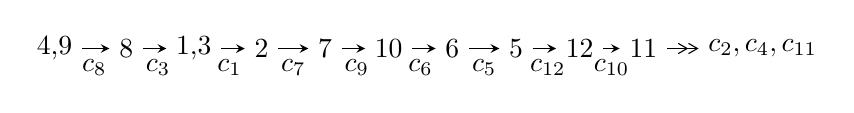
\begin{tikzpicture}[x=23pt, y=7pt]
	% node
	\node (A0) at (-1/8, 0) {4,9};
	\node (A1) at (1, 0) {8};
	\node (A2) at (33/16, 0) {1,3};
	\node (A3) at (25/8, 0) {2};
	\node (A4) at (33/8, 0) {7};
	\node (A5) at (41/8, 0) {10};
	\node (A6) at (49/8, 0) {6};
	\node (A7) at (57/8, 0) {5};
	\node (A8) at (65/8, 0) {12};
	\node (A9) at (73/8, 0) {11};
	\node (C1) at (1/2, -1) {$c_{8}$};
	\node (C2) at (3/2, -1) {$c_{3}$};
	\node (C3) at (21/8, -1) {$c_{1}$};
	\node (C4) at (29/8, -1) {$c_{7}$};
	\node (C5) at (37/8, -1) {$c_{9}$};
	\node (C6) at (45/8, -1) {$c_{6}$};
	\node (C7) at (53/8, -1) {$c_{5}$};
	\node (C8) at (61/8, -1) {$c_{12}$};
	\node (C9) at (69/8, -1) {$c_{10}$};
	\node (A10) at (11, 0) {$c_{2},c_{4},c_{11}$};

	% edge
	\draw[->,>=stealth]	
	(A0) edge (A1) (A1) edge (A2) (A2) edge (A3) (A3) edge (A4) (A4) edge (A5) (A5) edge (A6) (A6) edge (A7) (A7) edge (A8) (A8) edge (A9) ;
	\draw[->>,>={angle 60}]	
	(A9) edge (A10);
\end{tikzpicture} \\ 

\end{tabular} \\

\footnotetext{
The image of knot diagram is generated by the software ``\textbf{Draw programme}" developed by Andrew Bartholomew(\url{http://www.layer8.co.uk/maths/draw/index.htm\#Running-draw}), where we modified some parts for our purpose(\url{https://github.com/CATsTAILs/LinksPainter}).
}\phantom \\ \newline 
\centering \textbf{Ideals for irreducible components\footnotemark of $X_{\text{par}}$} 
 
\begin{align*}
I^u_{1}&=\langle 
- u^{23}- u^{22}+\cdots+4 b+1,\;- u^6+u^4-2 u^2+a+1,\;u^{24}- u^{23}+\cdots-3 u^2+1\rangle \\
I^u_{2}&=\langle 
-1.28182\times10^{16} u^{51}-5.11407\times10^{16} u^{50}+\cdots+3.64498\times10^{17} b+4.59559\times10^{17},\\
\phantom{I^u_{2}}&\phantom{= \langle  }2.08375\times10^{17} u^{51}-4.62594\times10^{17} u^{50}+\cdots+7.28997\times10^{17} a+2.74422\times10^{18},\;u^{52}-2 u^{51}+\cdots+20 u+4\rangle \\
I^u_{3}&=\langle 
u^3+u^2+b,\;- u^2+a+1,\;u^4- u^2+1\rangle \\
I^u_{4}&=\langle 
b- u,\;a,\;u^{12}- u^{11}-2 u^{10}+3 u^9+2 u^8-5 u^7+u^6+3 u^5-2 u^4+2 u^2-2 u+1\rangle \\
I^u_{5}&=\langle 
a^3 u^2+8 a^3 u+5 a^2 u^2+10 a^3+17 a^2 u-57 u^2 a+27 a^2-42 a u-60 u^2+46 b+5 a-43 u-48,\\
\phantom{I^u_{5}}&\phantom{= \langle  }a^4-2 a^3 u-2 a^2 u^2- a^2 u-6 u^2 a- a^2+3 u^2+6 a+4 u-1,\;u^3+u^2-1\rangle \\
I^u_{6}&=\langle 
b- u,\;a,\;u^3+u^2-1\rangle \\
I^u_{7}&=\langle 
- u^2+b- u+1,\;a-1,\;u^4- u^2+1\rangle \\
I^u_{8}&=\langle 
u^2+b- u,\;- u^2+a+1,\;u^4- u^2+1\rangle \\
I^u_{9}&=\langle 
u^3- u^2+b+1,\;a-1,\;u^4- u^2+1\rangle \\
\\
\end{align*}
\raggedright * 9 irreducible components of $\dim_{\mathbb{C}}=0$, with total 119 representations.\\
\footnotetext{All coefficients of polynomials are rational numbers. But the coefficients are sometimes approximated in decimal forms when there is not enough margin.}
\newpage
\renewcommand{\arraystretch}{1}
\centering \section*{I. $I^u_{1}= \langle - u^{23}- u^{22}+\cdots+4 b+1,\;- u^6+u^4-2 u^2+a+1,\;u^{24}- u^{23}+\cdots-3 u^2+1 \rangle$}
\flushleft \textbf{(i) Arc colorings}\\
\begin{tabular}{m{7pt} m{180pt} m{7pt} m{180pt} }
\flushright $a_{4}=$&$\begin{pmatrix}0\\u\end{pmatrix}$ \\
\flushright $a_{9}=$&$\begin{pmatrix}1\\0\end{pmatrix}$ \\
\flushright $a_{8}=$&$\begin{pmatrix}1\\u^2\end{pmatrix}$ \\
\flushright $a_{1}=$&$\begin{pmatrix}u^6- u^4+2 u^2-1\\\frac{1}{4} u^{23}+\frac{1}{4} u^{22}+\cdots+2 u^2-\frac{1}{4}\end{pmatrix}$ \\
\flushright $a_{3}=$&$\begin{pmatrix}- u\\- u^3+u\end{pmatrix}$ \\
\flushright $a_{2}=$&$\begin{pmatrix}-\frac{1}{4} u^{23}+u^{21}+\cdots+\frac{1}{4} u-\frac{1}{2}\\\frac{1}{2} u^{23}+\frac{1}{2} u^{22}+\cdots+2 u^2-\frac{1}{2}\end{pmatrix}$ \\
\flushright $a_{7}=$&$\begin{pmatrix}- u^2+1\\u^2\end{pmatrix}$ \\
\flushright $a_{10}=$&$\begin{pmatrix}u^4- u^2+1\\- u^4\end{pmatrix}$ \\
\flushright $a_{6}=$&$\begin{pmatrix}\frac{1}{4} u^{23}- u^{21}+\cdots-\frac{1}{4} u+\frac{1}{2}\\\frac{1}{4} u^{22}-\frac{1}{2} u^{21}+\cdots-\frac{1}{4} u-\frac{3}{4}\end{pmatrix}$ \\
\flushright $a_{5}=$&$\begin{pmatrix}u\\-\frac{1}{4} u^{23}+\frac{1}{4} u^{22}+\cdots+\frac{3}{2} u+\frac{1}{4}\end{pmatrix}$ \\
\flushright $a_{12}=$&$\begin{pmatrix}u^2-1\\\frac{1}{4} u^{23}+\frac{1}{4} u^{22}+\cdots+2 u^2-\frac{1}{4}\end{pmatrix}$ \\
\flushright $a_{11}=$&$\begin{pmatrix}1\\-\frac{1}{4} u^{23}+u^{21}+\cdots+\frac{1}{4} u+\frac{1}{2}\end{pmatrix}$\\&\end{tabular}
\flushleft \textbf{(ii) Obstruction class $= -1$}\\~\\
\flushleft \textbf{(iii) Cusp Shapes $= u^{23}-\frac{5}{2} u^{22}+6 u^{20}- u^{19}-21 u^{18}+19 u^{17}+29 u^{16}-\frac{95}{2} u^{15}-43 u^{14}+\frac{193}{2} u^{13}+31 u^{12}-\frac{295}{2} u^{11}-3 u^{10}+161 u^9-\frac{35}{2} u^8-\frac{311}{2} u^7+\frac{95}{2} u^6+95 u^5-\frac{61}{2} u^4-36 u^3+\frac{7}{2} u^2+\frac{23}{2} u+\frac{15}{2}$}\\~\\
\newpage\renewcommand{\arraystretch}{1}
\flushleft \textbf{(iv) u-Polynomials at the component}\newline \\
\begin{tabular}{m{50pt}|m{274pt}}
Crossings & \hspace{64pt}u-Polynomials at each crossing \\
\hline $$\begin{aligned}c_{1}\end{aligned}$$&$\begin{aligned}
&u^{24}+12 u^{23}+\cdots+56 u+16
\end{aligned}$\\
\hline $$\begin{aligned}c_{2},c_{5}\end{aligned}$$&$\begin{aligned}
&u^{24}+4 u^{23}+\cdots+12 u+4
\end{aligned}$\\
\hline $$\begin{aligned}c_{3},c_{4},c_{8}\\c_{11}\end{aligned}$$&$\begin{aligned}
&u^{24}- u^{23}+\cdots-3 u^2+1
\end{aligned}$\\
\hline $$\begin{aligned}c_{6}\end{aligned}$$&$\begin{aligned}
&u^{24}+12 u^{23}+\cdots+876 u+188
\end{aligned}$\\
\hline $$\begin{aligned}c_{7},c_{9},c_{10}\\c_{12}\end{aligned}$$&$\begin{aligned}
&u^{24}-7 u^{23}+\cdots-6 u+1
\end{aligned}$\\
\hline
\end{tabular}\\~\\
\newpage\renewcommand{\arraystretch}{1}
\flushleft \textbf{(v) Riley Polynomials at the component}\newline \\
\begin{tabular}{m{50pt}|m{274pt}}
Crossings & \hspace{64pt}Riley Polynomials at each crossing \\
\hline $$\begin{aligned}c_{1}\end{aligned}$$&$\begin{aligned}
&y^{24}+24 y^{22}+\cdots+1760 y+256
\end{aligned}$\\
\hline $$\begin{aligned}c_{2},c_{5}\end{aligned}$$&$\begin{aligned}
&y^{24}-12 y^{23}+\cdots-56 y+16
\end{aligned}$\\
\hline $$\begin{aligned}c_{3},c_{4},c_{8}\\c_{11}\end{aligned}$$&$\begin{aligned}
&y^{24}-7 y^{23}+\cdots-6 y+1
\end{aligned}$\\
\hline $$\begin{aligned}c_{6}\end{aligned}$$&$\begin{aligned}
&y^{24}+12 y^{23}+\cdots-37560 y+35344
\end{aligned}$\\
\hline $$\begin{aligned}c_{7},c_{9},c_{10}\\c_{12}\end{aligned}$$&$\begin{aligned}
&y^{24}+25 y^{23}+\cdots+6 y+1
\end{aligned}$\\
\hline
\end{tabular}\\~\\
\newpage\flushleft \textbf{(vi) Complex Volumes and Cusp Shapes}
$$\begin{array}{c|c|c}  
\text{Solutions to }I^u_{1}& \I (\text{vol} + \sqrt{-1}CS) & \text{Cusp shape}\\
 \hline 
\begin{aligned}
u &= -0.997654 + 0.063385 I \\
a &= \phantom{-}0.942467 - 0.373018 I \\
b &= \phantom{-}0.114843 + 0.496939 I\end{aligned}
 & \phantom{-}5.25543 - 0.92360 I & \phantom{-}15.9667 + 0.9405 I \\ \hline\begin{aligned}
u &= -0.997654 - 0.063385 I \\
a &= \phantom{-}0.942467 + 0.373018 I \\
b &= \phantom{-}0.114843 - 0.496939 I\end{aligned}
 & \phantom{-}5.25543 + 0.92360 I & \phantom{-}15.9667 - 0.9405 I \\ \hline\begin{aligned}
u &= \phantom{-}1.001330 + 0.130771 I \\
a &= \phantom{-}0.822888 + 0.752742 I \\
b &= \phantom{-}0.402636 - 1.030140 I\end{aligned}
 & \phantom{-}3.57553 + 5.62812 I & \phantom{-}12.5450 - 6.6163 I \\ \hline\begin{aligned}
u &= \phantom{-}1.001330 - 0.130771 I \\
a &= \phantom{-}0.822888 - 0.752742 I \\
b &= \phantom{-}0.402636 + 1.030140 I\end{aligned}
 & \phantom{-}3.57553 - 5.62812 I & \phantom{-}12.5450 + 6.6163 I \\ \hline\begin{aligned}
u &= -0.760211 + 0.865552 I \\
a &= \phantom{-}1.24479 - 0.91941 I \\
b &= -2.02625 - 0.25873 I\end{aligned}
 & -7.41712 - 0.40141 I & \phantom{-}2.13735 + 2.27627 I \\ \hline\begin{aligned}
u &= -0.760211 - 0.865552 I \\
a &= \phantom{-}1.24479 + 0.91941 I \\
b &= -2.02625 + 0.25873 I\end{aligned}
 & -7.41712 + 0.40141 I & \phantom{-}2.13735 - 2.27627 I \\ \hline\begin{aligned}
u &= \phantom{-}0.729818 + 0.904919 I \\
a &= \phantom{-}1.56496 + 1.41813 I \\
b &= -2.37154 + 0.16884 I\end{aligned}
 & -10.52250 - 4.79311 I & -0.73258 + 1.28832 I \\ \hline\begin{aligned}
u &= \phantom{-}0.729818 - 0.904919 I \\
a &= \phantom{-}1.56496 - 1.41813 I \\
b &= -2.37154 - 0.16884 I\end{aligned}
 & -10.52250 + 4.79311 I & -0.73258 - 1.28832 I \\ \hline\begin{aligned}
u &= \phantom{-}0.925994 + 0.739498 I \\
a &= -0.317422 - 0.284084 I \\
b &= -0.032960 - 1.025040 I\end{aligned}
 & -2.70773 + 8.50857 I & \phantom{-}3.70396 - 8.56767 I \\ \hline\begin{aligned}
u &= \phantom{-}0.925994 - 0.739498 I \\
a &= -0.317422 + 0.284084 I \\
b &= -0.032960 + 1.025040 I\end{aligned}
 & -2.70773 - 8.50857 I & \phantom{-}3.70396 + 8.56767 I\\
 \hline 
 \end{array}$$\newpage$$\begin{array}{c|c|c}  
\text{Solutions to }I^u_{1}& \I (\text{vol} + \sqrt{-1}CS) & \text{Cusp shape}\\
 \hline 
\begin{aligned}
u &= \phantom{-}0.820795 + 0.890761 I \\
a &= \phantom{-}1.65081 + 0.21101 I \\
b &= -1.82529 + 0.81637 I\end{aligned}
 & -12.04400 + 4.45797 I & -1.81976 - 4.80562 I \\ \hline\begin{aligned}
u &= \phantom{-}0.820795 - 0.890761 I \\
a &= \phantom{-}1.65081 - 0.21101 I \\
b &= -1.82529 - 0.81637 I\end{aligned}
 & -12.04400 - 4.45797 I & -1.81976 + 4.80562 I \\ \hline\begin{aligned}
u &= \phantom{-}1.024520 + 0.763888 I \\
a &= -1.15966 - 1.14324 I \\
b &= \phantom{-}2.19721 - 0.55212 I\end{aligned}
 & -5.73077 + 11.79410 I & \phantom{-}4.86199 - 7.29279 I \\ \hline\begin{aligned}
u &= \phantom{-}1.024520 - 0.763888 I \\
a &= -1.15966 + 1.14324 I \\
b &= \phantom{-}2.19721 + 0.55212 I\end{aligned}
 & -5.73077 - 11.79410 I & \phantom{-}4.86199 + 7.29279 I \\ \hline\begin{aligned}
u &= -1.004430 + 0.806604 I \\
a &= -0.56218 + 1.55066 I \\
b &= \phantom{-}1.64632 - 0.45435 I\end{aligned}
 & -10.85360 - 8.18091 I & -0.32980 + 5.06079 I \\ \hline\begin{aligned}
u &= -1.004430 - 0.806604 I \\
a &= -0.56218 - 1.55066 I \\
b &= \phantom{-}1.64632 + 0.45435 I\end{aligned}
 & -10.85360 + 8.18091 I & -0.32980 - 5.06079 I \\ \hline\begin{aligned}
u &= -0.602609 + 0.358517 I \\
a &= -0.517620 - 0.652115 I \\
b &= \phantom{-}0.102178 - 1.019880 I\end{aligned}
 & \phantom{-}0.06490 - 4.25573 I & \phantom{-}5.05969 + 5.51828 I \\ \hline\begin{aligned}
u &= -0.602609 - 0.358517 I \\
a &= -0.517620 + 0.652115 I \\
b &= \phantom{-}0.102178 + 1.019880 I\end{aligned}
 & \phantom{-}0.06490 + 4.25573 I & \phantom{-}5.05969 - 5.51828 I \\ \hline\begin{aligned}
u &= -1.051550 + 0.766917 I \\
a &= -1.53210 + 1.34344 I \\
b &= \phantom{-}2.87795 + 0.47141 I\end{aligned}
 & -8.4633 - 17.2201 I & \phantom{-}2.43977 + 10.58669 I \\ \hline\begin{aligned}
u &= -1.051550 - 0.766917 I \\
a &= -1.53210 - 1.34344 I \\
b &= \phantom{-}2.87795 - 0.47141 I\end{aligned}
 & -8.4633 + 17.2201 I & \phantom{-}2.43977 - 10.58669 I\\
 \hline 
 \end{array}$$\newpage$$\begin{array}{c|c|c}  
\text{Solutions to }I^u_{1}& \I (\text{vol} + \sqrt{-1}CS) & \text{Cusp shape}\\
 \hline 
\begin{aligned}
u &= \phantom{-}0.638863 + 0.153437 I \\
a &= -0.327734 + 0.320762 I \\
b &= \phantom{-}0.626252 + 0.329284 I\end{aligned}
 & \phantom{-}1.105580 + 0.097930 I & \phantom{-}9.88722 - 0.56674 I \\ \hline\begin{aligned}
u &= \phantom{-}0.638863 - 0.153437 I \\
a &= -0.327734 - 0.320762 I \\
b &= \phantom{-}0.626252 - 0.329284 I\end{aligned}
 & \phantom{-}1.105580 - 0.097930 I & \phantom{-}9.88722 + 0.56674 I \\ \hline\begin{aligned}
u &= -0.224865 + 0.471112 I \\
a &= -1.309200 - 0.505527 I \\
b &= -0.211349 - 0.055814 I\end{aligned}
 & -1.61046 + 1.10126 I & -1.71956 - 0.90297 I \\ \hline\begin{aligned}
u &= -0.224865 - 0.471112 I \\
a &= -1.309200 + 0.505527 I \\
b &= -0.211349 + 0.055814 I\end{aligned}
 & -1.61046 - 1.10126 I & -1.71956 + 0.90297 I\\
 \hline 
 \end{array}$$\newpage\newpage\renewcommand{\arraystretch}{1}
\centering \section*{II. $I^u_{2}= \langle -1.28\times10^{16} u^{51}-5.11\times10^{16} u^{50}+\cdots+3.64\times10^{17} b+4.60\times10^{17},\;2.08\times10^{17} u^{51}-4.63\times10^{17} u^{50}+\cdots+7.29\times10^{17} a+2.74\times10^{18},\;u^{52}-2 u^{51}+\cdots+20 u+4 \rangle$}
\flushleft \textbf{(i) Arc colorings}\\
\begin{tabular}{m{7pt} m{180pt} m{7pt} m{180pt} }
\flushright $a_{4}=$&$\begin{pmatrix}0\\u\end{pmatrix}$ \\
\flushright $a_{9}=$&$\begin{pmatrix}1\\0\end{pmatrix}$ \\
\flushright $a_{8}=$&$\begin{pmatrix}1\\u^2\end{pmatrix}$ \\
\flushright $a_{1}=$&$\begin{pmatrix}-0.285839 u^{51}+0.634563 u^{50}+\cdots-11.9888 u-3.76438\\0.0351666 u^{51}+0.140304 u^{50}+\cdots-7.18667 u-1.26080\end{pmatrix}$ \\
\flushright $a_{3}=$&$\begin{pmatrix}- u\\- u^3+u\end{pmatrix}$ \\
\flushright $a_{2}=$&$\begin{pmatrix}-0.376087 u^{51}+0.637127 u^{50}+\cdots-10.2579 u-3.06437\\-0.0536490 u^{51}+0.328407 u^{50}+\cdots-4.99796 u-1.24908\end{pmatrix}$ \\
\flushright $a_{7}=$&$\begin{pmatrix}- u^2+1\\u^2\end{pmatrix}$ \\
\flushright $a_{10}=$&$\begin{pmatrix}u^4- u^2+1\\- u^4\end{pmatrix}$ \\
\flushright $a_{6}=$&$\begin{pmatrix}-0.0501715 u^{51}+0.417802 u^{50}+\cdots-9.11537 u-4.14850\\-0.102327 u^{51}-0.0485043 u^{50}+\cdots-8.90760 u-1.99867\end{pmatrix}$ \\
\flushright $a_{5}=$&$\begin{pmatrix}0.0611096 u^{51}-0.333673 u^{50}+\cdots+7.08230 u-1.32447\\-0.120328 u^{51}+0.230313 u^{50}+\cdots+6.03865 u+0.284922\end{pmatrix}$ \\
\flushright $a_{12}=$&$\begin{pmatrix}-0.336174 u^{51}+0.534328 u^{50}+\cdots-6.12727 u-2.93706\\0.185608 u^{51}+0.186049 u^{50}+\cdots-7.63784 u-1.44011\end{pmatrix}$ \\
\flushright $a_{11}=$&$\begin{pmatrix}-0.222742 u^{51}+0.513738 u^{50}+\cdots+5.05004 u+4.21170\\0.221796 u^{51}-0.742510 u^{50}+\cdots-0.144816 u+0.763127\end{pmatrix}$\\&\end{tabular}
\flushleft \textbf{(ii) Obstruction class $= -1$}\\~\\
\flushleft \textbf{(iii) Cusp Shapes $= \frac{175172589829383178}{91124580510363867} u^{51}-\frac{434551767463876444}{91124580510363867} u^{50}+\cdots+\frac{784093020302745154}{91124580510363867} u+\frac{353320257970419306}{30374860170121289}$}\\~\\
\newpage\renewcommand{\arraystretch}{1}
\flushleft \textbf{(iv) u-Polynomials at the component}\newline \\
\begin{tabular}{m{50pt}|m{274pt}}
Crossings & \hspace{64pt}u-Polynomials at each crossing \\
\hline $$\begin{aligned}c_{1}\end{aligned}$$&$\begin{aligned}
&(u^{26}+15 u^{25}+\cdots+4 u+1)^{2}
\end{aligned}$\\
\hline $$\begin{aligned}c_{2},c_{5}\end{aligned}$$&$\begin{aligned}
&(u^{26}- u^{25}+\cdots-2 u^2+1)^{2}
\end{aligned}$\\
\hline $$\begin{aligned}c_{3},c_{4},c_{8}\\c_{11}\end{aligned}$$&$\begin{aligned}
&u^{52}-2 u^{51}+\cdots+20 u+4
\end{aligned}$\\
\hline $$\begin{aligned}c_{6}\end{aligned}$$&$\begin{aligned}
&(u^{26}-3 u^{25}+\cdots+4 u+1)^{2}
\end{aligned}$\\
\hline $$\begin{aligned}c_{7},c_{9},c_{10}\\c_{12}\end{aligned}$$&$\begin{aligned}
&u^{52}-16 u^{51}+\cdots-152 u+16
\end{aligned}$\\
\hline
\end{tabular}\\~\\
\newpage\renewcommand{\arraystretch}{1}
\flushleft \textbf{(v) Riley Polynomials at the component}\newline \\
\begin{tabular}{m{50pt}|m{274pt}}
Crossings & \hspace{64pt}Riley Polynomials at each crossing \\
\hline $$\begin{aligned}c_{1}\end{aligned}$$&$\begin{aligned}
&(y^{26}-3 y^{25}+\cdots-16 y+1)^{2}
\end{aligned}$\\
\hline $$\begin{aligned}c_{2},c_{5}\end{aligned}$$&$\begin{aligned}
&(y^{26}-15 y^{25}+\cdots-4 y+1)^{2}
\end{aligned}$\\
\hline $$\begin{aligned}c_{3},c_{4},c_{8}\\c_{11}\end{aligned}$$&$\begin{aligned}
&y^{52}-16 y^{51}+\cdots-152 y+16
\end{aligned}$\\
\hline $$\begin{aligned}c_{6}\end{aligned}$$&$\begin{aligned}
&(y^{26}+21 y^{25}+\cdots-68 y+1)^{2}
\end{aligned}$\\
\hline $$\begin{aligned}c_{7},c_{9},c_{10}\\c_{12}\end{aligned}$$&$\begin{aligned}
&y^{52}+40 y^{51}+\cdots+78048 y+256
\end{aligned}$\\
\hline
\end{tabular}\\~\\
\newpage\flushleft \textbf{(vi) Complex Volumes and Cusp Shapes}
$$\begin{array}{c|c|c}  
\text{Solutions to }I^u_{2}& \I (\text{vol} + \sqrt{-1}CS) & \text{Cusp shape}\\
 \hline 
\begin{aligned}
u &= \phantom{-}0.752589 + 0.686692 I \\
a &= -1.19861 - 1.00203 I \\
b &= \phantom{-}1.75066 - 0.28301 I\end{aligned}
 & \phantom{-}0.134724 - 0.617454 I & \phantom{-}7.60333 + 0.92062 I \\ \hline\begin{aligned}
u &= \phantom{-}0.752589 - 0.686692 I \\
a &= -1.19861 + 1.00203 I \\
b &= \phantom{-}1.75066 + 0.28301 I\end{aligned}
 & \phantom{-}0.134724 + 0.617454 I & \phantom{-}7.60333 - 0.92062 I \\ \hline\begin{aligned}
u &= \phantom{-}1.021920 + 0.291673 I \\
a &= -0.675586 - 0.356154 I \\
b &= \phantom{-}0.0136506 - 0.1110620 I\end{aligned}
 & \phantom{-}0.134724 + 0.617454 I & \phantom{-}7.60333 - 0.92062 I \\ \hline\begin{aligned}
u &= \phantom{-}1.021920 - 0.291673 I \\
a &= -0.675586 + 0.356154 I \\
b &= \phantom{-}0.0136506 + 0.1110620 I\end{aligned}
 & \phantom{-}0.134724 - 0.617454 I & \phantom{-}7.60333 + 0.92062 I \\ \hline\begin{aligned}
u &= -0.842250 + 0.401014 I \\
a &= -0.301397 + 0.041356 I \\
b &= -0.014640 - 1.010940 I\end{aligned}
 & \phantom{-}0.11473 - 4.15162 I & \phantom{-}6.01126 + 6.89813 I \\ \hline\begin{aligned}
u &= -0.842250 - 0.401014 I \\
a &= -0.301397 - 0.041356 I \\
b &= -0.014640 + 1.010940 I\end{aligned}
 & \phantom{-}0.11473 + 4.15162 I & \phantom{-}6.01126 - 6.89813 I \\ \hline\begin{aligned}
u &= -0.752492 + 0.788189 I \\
a &= -1.69455 + 1.94272 I \\
b &= \phantom{-}2.70085 - 0.03238 I\end{aligned}
 & -2.50569 + 4.90020 I & \phantom{-}3.66047 - 4.25570 I \\ \hline\begin{aligned}
u &= -0.752492 - 0.788189 I \\
a &= -1.69455 - 1.94272 I \\
b &= \phantom{-}2.70085 + 0.03238 I\end{aligned}
 & -2.50569 - 4.90020 I & \phantom{-}3.66047 + 4.25570 I \\ \hline\begin{aligned}
u &= \phantom{-}0.951867 + 0.554822 I \\
a &= -1.110860 + 0.329191 I \\
b &= \phantom{-}0.36805 - 1.46263 I\end{aligned}
 & -0.330999\phantom{ +0.000000I} & \phantom{-}4.51777 + 0. I\phantom{ +0.000000I} \\ \hline\begin{aligned}
u &= \phantom{-}0.951867 - 0.554822 I \\
a &= -1.110860 - 0.329191 I \\
b &= \phantom{-}0.36805 + 1.46263 I\end{aligned}
 & -0.330999\phantom{ +0.000000I} & \phantom{-}4.51777 + 0. I\phantom{ +0.000000I}\\
 \hline 
 \end{array}$$\newpage$$\begin{array}{c|c|c}  
\text{Solutions to }I^u_{2}& \I (\text{vol} + \sqrt{-1}CS) & \text{Cusp shape}\\
 \hline 
\begin{aligned}
u &= -1.084340 + 0.227015 I \\
a &= \phantom{-}0.703611 - 0.413455 I \\
b &= \phantom{-}0.194210 - 0.006182 I\end{aligned}
 & \phantom{-}0.74787 - 5.97219 I & \phantom{-}9.15925 + 6.03254 I \\ \hline\begin{aligned}
u &= -1.084340 - 0.227015 I \\
a &= \phantom{-}0.703611 + 0.413455 I \\
b &= \phantom{-}0.194210 + 0.006182 I\end{aligned}
 & \phantom{-}0.74787 + 5.97219 I & \phantom{-}9.15925 - 6.03254 I \\ \hline\begin{aligned}
u &= -0.885563 + 0.095980 I \\
a &= \phantom{-}1.47605 + 0.13629 I \\
b &= -0.239465 - 1.096400 I\end{aligned}
 & \phantom{-}2.16312 - 4.62114 I & \phantom{-}11.65491 + 5.89029 I \\ \hline\begin{aligned}
u &= -0.885563 - 0.095980 I \\
a &= \phantom{-}1.47605 - 0.13629 I \\
b &= -0.239465 + 1.096400 I\end{aligned}
 & \phantom{-}2.16312 + 4.62114 I & \phantom{-}11.65491 - 5.89029 I \\ \hline\begin{aligned}
u &= -0.988091 + 0.542376 I \\
a &= \phantom{-}0.473259 + 0.644867 I \\
b &= \phantom{-}0.136840 - 1.204680 I\end{aligned}
 & -1.24430 - 4.51893 I & \phantom{-}1.06028 + 5.49831 I \\ \hline\begin{aligned}
u &= -0.988091 - 0.542376 I \\
a &= \phantom{-}0.473259 - 0.644867 I \\
b &= \phantom{-}0.136840 + 1.204680 I\end{aligned}
 & -1.24430 + 4.51893 I & \phantom{-}1.06028 - 5.49831 I \\ \hline\begin{aligned}
u &= \phantom{-}0.652457 + 0.571498 I \\
a &= \phantom{-}0.98577 - 1.47704 I \\
b &= \phantom{-}0.58799 + 1.32773 I\end{aligned}
 & -1.24430 + 4.51893 I & \phantom{-}1.06028 - 5.49831 I \\ \hline\begin{aligned}
u &= \phantom{-}0.652457 - 0.571498 I \\
a &= \phantom{-}0.98577 + 1.47704 I \\
b &= \phantom{-}0.58799 - 1.32773 I\end{aligned}
 & -1.24430 - 4.51893 I & \phantom{-}1.06028 + 5.49831 I \\ \hline\begin{aligned}
u &= \phantom{-}0.722344 + 0.873653 I \\
a &= -1.27009 - 0.90834 I \\
b &= \phantom{-}2.02407 - 0.21519 I\end{aligned}
 & -6.66680 - 5.70836 I & \phantom{-}3.28436 + 2.61089 I \\ \hline\begin{aligned}
u &= \phantom{-}0.722344 - 0.873653 I \\
a &= -1.27009 + 0.90834 I \\
b &= \phantom{-}2.02407 + 0.21519 I\end{aligned}
 & -6.66680 + 5.70836 I & \phantom{-}3.28436 - 2.61089 I\\
 \hline 
 \end{array}$$\newpage$$\begin{array}{c|c|c}  
\text{Solutions to }I^u_{2}& \I (\text{vol} + \sqrt{-1}CS) & \text{Cusp shape}\\
 \hline 
\begin{aligned}
u &= \phantom{-}0.971674 + 0.598016 I \\
a &= -0.392194 - 0.140230 I \\
b &= \phantom{-}0.003048 - 0.949049 I\end{aligned}
 & \phantom{-}2.16312 + 4.62114 I & \phantom{-}11.65491 - 5.89029 I \\ \hline\begin{aligned}
u &= \phantom{-}0.971674 - 0.598016 I \\
a &= -0.392194 + 0.140230 I \\
b &= \phantom{-}0.003048 + 0.949049 I\end{aligned}
 & \phantom{-}2.16312 - 4.62114 I & \phantom{-}11.65491 + 5.89029 I \\ \hline\begin{aligned}
u &= -0.695608 + 0.907900 I \\
a &= -1.66112 + 1.35074 I \\
b &= \phantom{-}2.39253 + 0.23778 I\end{aligned}
 & -9.5709 + 11.0305 I & \phantom{-}0.68896 - 6.00028 I \\ \hline\begin{aligned}
u &= -0.695608 - 0.907900 I \\
a &= -1.66112 - 1.35074 I \\
b &= \phantom{-}2.39253 - 0.23778 I\end{aligned}
 & -9.5709 - 11.0305 I & \phantom{-}0.68896 + 6.00028 I \\ \hline\begin{aligned}
u &= -0.128928 + 0.836166 I \\
a &= \phantom{-}0.704339 - 0.655474 I \\
b &= -0.253889 - 0.601697 I\end{aligned}
 & -6.22742 - 7.20928 I & -0.73612 + 6.27610 I \\ \hline\begin{aligned}
u &= -0.128928 - 0.836166 I \\
a &= \phantom{-}0.704339 + 0.655474 I \\
b &= -0.253889 + 0.601697 I\end{aligned}
 & -6.22742 + 7.20928 I & -0.73612 - 6.27610 I \\ \hline\begin{aligned}
u &= \phantom{-}0.834456 + 0.812598 I \\
a &= \phantom{-}1.21182 + 1.89134 I \\
b &= -2.39545 - 0.28919 I\end{aligned}
 & -6.53686 - 1.23377 I & -1.59190 + 0.83965 I \\ \hline\begin{aligned}
u &= \phantom{-}0.834456 - 0.812598 I \\
a &= \phantom{-}1.21182 - 1.89134 I \\
b &= -2.39545 + 0.28919 I\end{aligned}
 & -6.53686 + 1.23377 I & -1.59190 - 0.83965 I \\ \hline\begin{aligned}
u &= \phantom{-}0.054522 + 0.827933 I \\
a &= -0.782373 - 0.644964 I \\
b &= \phantom{-}0.272506 - 0.513614 I\end{aligned}
 & -6.53686 + 1.23377 I & -1.59190 - 0.83965 I \\ \hline\begin{aligned}
u &= \phantom{-}0.054522 - 0.827933 I \\
a &= -0.782373 + 0.644964 I \\
b &= \phantom{-}0.272506 + 0.513614 I\end{aligned}
 & -6.53686 - 1.23377 I & -1.59190 + 0.83965 I\\
 \hline 
 \end{array}$$\newpage$$\begin{array}{c|c|c}  
\text{Solutions to }I^u_{2}& \I (\text{vol} + \sqrt{-1}CS) & \text{Cusp shape}\\
 \hline 
\begin{aligned}
u &= -1.139850 + 0.271378 I \\
a &= -0.431580 + 0.818565 I \\
b &= -0.237751 - 0.669102 I\end{aligned}
 & -2.50569 - 4.90020 I & \phantom{-}3.66047 + 4.25570 I \\ \hline\begin{aligned}
u &= -1.139850 - 0.271378 I \\
a &= -0.431580 - 0.818565 I \\
b &= -0.237751 + 0.669102 I\end{aligned}
 & -2.50569 + 4.90020 I & \phantom{-}3.66047 - 4.25570 I \\ \hline\begin{aligned}
u &= \phantom{-}0.955556 + 0.693925 I \\
a &= -1.33481 - 1.07208 I \\
b &= \phantom{-}2.06526 - 0.70643 I\end{aligned}
 & \phantom{-}0.74787 + 5.97219 I & \phantom{-}9.15925 - 6.03254 I \\ \hline\begin{aligned}
u &= \phantom{-}0.955556 - 0.693925 I \\
a &= -1.33481 + 1.07208 I \\
b &= \phantom{-}2.06526 + 0.70643 I\end{aligned}
 & \phantom{-}0.74787 - 5.97219 I & \phantom{-}9.15925 + 6.03254 I \\ \hline\begin{aligned}
u &= \phantom{-}1.160440 + 0.222987 I \\
a &= \phantom{-}0.476162 + 0.877504 I \\
b &= \phantom{-}0.345484 - 0.648450 I\end{aligned}
 & -1.81559 + 10.65820 I & \phantom{-}6.00000 - 9.11948 I \\ \hline\begin{aligned}
u &= \phantom{-}1.160440 - 0.222987 I \\
a &= \phantom{-}0.476162 - 0.877504 I \\
b &= \phantom{-}0.345484 + 0.648450 I\end{aligned}
 & -1.81559 - 10.65820 I & \phantom{-}6.00000 + 9.11948 I \\ \hline\begin{aligned}
u &= -0.782234 + 0.897806 I \\
a &= -1.60548 + 0.09310 I \\
b &= \phantom{-}1.66931 + 0.79077 I\end{aligned}
 & -11.54940 + 1.88087 I & \phantom{-0.000000 } 0 \\ \hline\begin{aligned}
u &= -0.782234 - 0.897806 I \\
a &= -1.60548 - 0.09310 I \\
b &= \phantom{-}1.66931 - 0.79077 I\end{aligned}
 & -11.54940 - 1.88087 I & \phantom{-0.000000 } 0 \\ \hline\begin{aligned}
u &= -0.535320 + 0.606452 I \\
a &= -1.054240 - 0.782163 I \\
b &= -0.070591 + 0.734237 I\end{aligned}
 & -2.58244\phantom{ +0.000000I} & -2.20453 + 0. I\phantom{ +0.000000I} \\ \hline\begin{aligned}
u &= -0.535320 - 0.606452 I \\
a &= -1.054240 + 0.782163 I \\
b &= -0.070591 - 0.734237 I\end{aligned}
 & -2.58244\phantom{ +0.000000I} & -2.20453 + 0. I\phantom{ +0.000000I}\\
 \hline 
 \end{array}$$\newpage$$\begin{array}{c|c|c}  
\text{Solutions to }I^u_{2}& \I (\text{vol} + \sqrt{-1}CS) & \text{Cusp shape}\\
 \hline 
\begin{aligned}
u &= \phantom{-}0.934473 + 0.782146 I \\
a &= \phantom{-}2.03442 + 0.84782 I \\
b &= -2.58958 + 1.04646 I\end{aligned}
 & -6.22742 + 7.20928 I & \phantom{-0.000000 } 0. - 6.27610 I \\ \hline\begin{aligned}
u &= \phantom{-}0.934473 - 0.782146 I \\
a &= \phantom{-}2.03442 - 0.84782 I \\
b &= -2.58958 - 1.04646 I\end{aligned}
 & -6.22742 - 7.20928 I & \phantom{-0.000000 -}0. + 6.27610 I \\ \hline\begin{aligned}
u &= -0.978705 + 0.735947 I \\
a &= -2.06142 + 1.31787 I \\
b &= \phantom{-}3.02109 + 0.91961 I\end{aligned}
 & -1.81559 - 10.65820 I & \phantom{-}6.00000 + 9.11948 I \\ \hline\begin{aligned}
u &= -0.978705 - 0.735947 I \\
a &= -2.06142 - 1.31787 I \\
b &= \phantom{-}3.02109 - 0.91961 I\end{aligned}
 & -1.81559 + 10.65820 I & \phantom{-}6.00000 - 9.11948 I \\ \hline\begin{aligned}
u &= -1.001680 + 0.777271 I \\
a &= \phantom{-}1.16815 - 1.10223 I \\
b &= -2.16629 - 0.53914 I\end{aligned}
 & -6.66680 - 5.70836 I & \phantom{-0.000000 } 0 \\ \hline\begin{aligned}
u &= -1.001680 - 0.777271 I \\
a &= \phantom{-}1.16815 + 1.10223 I \\
b &= -2.16629 + 0.53914 I\end{aligned}
 & -6.66680 + 5.70836 I & \phantom{-0.000000 } 0 \\ \hline\begin{aligned}
u &= \phantom{-}0.978293 + 0.824595 I \\
a &= \phantom{-}0.66515 + 1.58276 I \\
b &= -1.76953 - 0.40279 I\end{aligned}
 & -11.54940 + 1.88087 I & \phantom{-0.000000 } 0 \\ \hline\begin{aligned}
u &= \phantom{-}0.978293 - 0.824595 I \\
a &= \phantom{-}0.66515 - 1.58276 I \\
b &= -1.76953 + 0.40279 I\end{aligned}
 & -11.54940 - 1.88087 I & \phantom{-0.000000 } 0 \\ \hline\begin{aligned}
u &= \phantom{-}1.034790 + 0.782497 I \\
a &= \phantom{-}1.58803 + 1.23418 I \\
b &= -2.80611 + 0.54589 I\end{aligned}
 & -9.5709 + 11.0305 I & \phantom{-0.000000 } 0 \\ \hline\begin{aligned}
u &= \phantom{-}1.034790 - 0.782497 I \\
a &= \phantom{-}1.58803 - 1.23418 I \\
b &= -2.80611 - 0.54589 I\end{aligned}
 & -9.5709 - 11.0305 I & \phantom{-0.000000 } 0\\
 \hline 
 \end{array}$$\newpage$$\begin{array}{c|c|c}  
\text{Solutions to }I^u_{2}& \I (\text{vol} + \sqrt{-1}CS) & \text{Cusp shape}\\
 \hline 
\begin{aligned}
u &= -0.210315 + 0.193461 I \\
a &= -0.16245 - 3.16407 I \\
b &= \phantom{-}0.497755 - 0.746437 I\end{aligned}
 & \phantom{-}0.11473 - 4.15162 I & \phantom{-}6.01126 + 6.89813 I \\ \hline\begin{aligned}
u &= -0.210315 - 0.193461 I \\
a &= -0.16245 + 3.16407 I \\
b &= \phantom{-}0.497755 + 0.746437 I\end{aligned}
 & \phantom{-}0.11473 + 4.15162 I & \phantom{-}6.01126 - 6.89813 I\\
 \hline 
 \end{array}$$\newpage\newpage\renewcommand{\arraystretch}{1}
\centering \section*{III. $I^u_{3}= \langle u^3+u^2+b,\;- u^2+a+1,\;u^4- u^2+1 \rangle$}
\flushleft \textbf{(i) Arc colorings}\\
\begin{tabular}{m{7pt} m{180pt} m{7pt} m{180pt} }
\flushright $a_{4}=$&$\begin{pmatrix}0\\u\end{pmatrix}$ \\
\flushright $a_{9}=$&$\begin{pmatrix}1\\0\end{pmatrix}$ \\
\flushright $a_{8}=$&$\begin{pmatrix}1\\u^2\end{pmatrix}$ \\
\flushright $a_{1}=$&$\begin{pmatrix}u^2-1\\- u^3- u^2\end{pmatrix}$ \\
\flushright $a_{3}=$&$\begin{pmatrix}- u\\- u^3+u\end{pmatrix}$ \\
\flushright $a_{2}=$&$\begin{pmatrix}u^3+u^2- u-1\\-2 u^3- u^2\end{pmatrix}$ \\
\flushright $a_{7}=$&$\begin{pmatrix}- u^2+1\\u^2\end{pmatrix}$ \\
\flushright $a_{10}=$&$\begin{pmatrix}0\\- u^2+1\end{pmatrix}$ \\
\flushright $a_{6}=$&$\begin{pmatrix}- u^3- u^2+u+1\\u^3+2 u^2-1\end{pmatrix}$ \\
\flushright $a_{5}=$&$\begin{pmatrix}u\\u^3- u-1\end{pmatrix}$ \\
\flushright $a_{12}=$&$\begin{pmatrix}u^2-1\\- u^3- u^2+1\end{pmatrix}$ \\
\flushright $a_{11}=$&$\begin{pmatrix}-1\\- u^3- u^2+u+2\end{pmatrix}$\\&\end{tabular}
\flushleft \textbf{(ii) Obstruction class $= 1$}\\~\\
\flushleft \textbf{(iii) Cusp Shapes $= -12 u^2+12$}\\~\\
\newpage\renewcommand{\arraystretch}{1}
\flushleft \textbf{(iv) u-Polynomials at the component}\newline \\
\begin{tabular}{m{50pt}|m{274pt}}
Crossings & \hspace{64pt}u-Polynomials at each crossing \\
\hline $$\begin{aligned}c_{1},c_{9},c_{12}\end{aligned}$$&$\begin{aligned}
&(u^2- u+1)^2
\end{aligned}$\\
\hline $$\begin{aligned}c_{2},c_{3},c_{4}\\c_{5},c_{6},c_{8}\\c_{11}\end{aligned}$$&$\begin{aligned}
&u^4- u^2+1
\end{aligned}$\\
\hline $$\begin{aligned}c_{7},c_{10}\end{aligned}$$&$\begin{aligned}
&(u^2+u+1)^2
\end{aligned}$\\
\hline
\end{tabular}\\~\\
\newpage\renewcommand{\arraystretch}{1}
\flushleft \textbf{(v) Riley Polynomials at the component}\newline \\
\begin{tabular}{m{50pt}|m{274pt}}
Crossings & \hspace{64pt}Riley Polynomials at each crossing \\
\hline $$\begin{aligned}c_{1},c_{7},c_{9}\\c_{10},c_{12}\end{aligned}$$&$\begin{aligned}
&(y^2+y+1)^2
\end{aligned}$\\
\hline $$\begin{aligned}c_{2},c_{3},c_{4}\\c_{5},c_{6},c_{8}\\c_{11}\end{aligned}$$&$\begin{aligned}
&(y^2- y+1)^2
\end{aligned}$\\
\hline
\end{tabular}\\~\\
\newpage\flushleft \textbf{(vi) Complex Volumes and Cusp Shapes}
$$\begin{array}{c|c|c}  
\text{Solutions to }I^u_{3}& \I (\text{vol} + \sqrt{-1}CS) & \text{Cusp shape}\\
 \hline 
\begin{aligned}
u &= \phantom{-}0.866025 + 0.500000 I \\
a &= -0.500000 + 0.866025 I \\
b &= -0.50000 - 1.86603 I\end{aligned}
 & \phantom{-0.000000 -}6.08965 I & \phantom{-}6.00000 - 10.39230 I \\ \hline\begin{aligned}
u &= \phantom{-}0.866025 - 0.500000 I \\
a &= -0.500000 - 0.866025 I \\
b &= -0.50000 + 1.86603 I\end{aligned}
 & \phantom{-0.000000 } -6.08965 I & \phantom{-}6.00000 + 10.39230 I \\ \hline\begin{aligned}
u &= -0.866025 + 0.500000 I \\
a &= -0.500000 - 0.866025 I \\
b &= -0.500000 - 0.133975 I\end{aligned}
 & \phantom{-0.000000 } -6.08965 I & \phantom{-}6.00000 + 10.39230 I \\ \hline\begin{aligned}
u &= -0.866025 - 0.500000 I \\
a &= -0.500000 + 0.866025 I \\
b &= -0.500000 + 0.133975 I\end{aligned}
 & \phantom{-0.000000 -}6.08965 I & \phantom{-}6.00000 - 10.39230 I\\
 \hline 
 \end{array}$$\newpage\newpage\renewcommand{\arraystretch}{1}
\centering \section*{IV. $I^u_{4}= \langle b- u,\;a,\;u^{12}- u^{11}+\cdots-2 u+1 \rangle$}
\flushleft \textbf{(i) Arc colorings}\\
\begin{tabular}{m{7pt} m{180pt} m{7pt} m{180pt} }
\flushright $a_{4}=$&$\begin{pmatrix}0\\u\end{pmatrix}$ \\
\flushright $a_{9}=$&$\begin{pmatrix}1\\0\end{pmatrix}$ \\
\flushright $a_{8}=$&$\begin{pmatrix}1\\u^2\end{pmatrix}$ \\
\flushright $a_{1}=$&$\begin{pmatrix}0\\u\end{pmatrix}$ \\
\flushright $a_{3}=$&$\begin{pmatrix}- u\\- u^3+u\end{pmatrix}$ \\
\flushright $a_{2}=$&$\begin{pmatrix}- u^3\\- u^5+u^3+u\end{pmatrix}$ \\
\flushright $a_{7}=$&$\begin{pmatrix}- u^2+1\\u^2\end{pmatrix}$ \\
\flushright $a_{10}=$&$\begin{pmatrix}u^4- u^2+1\\- u^4\end{pmatrix}$ \\
\flushright $a_{6}=$&$\begin{pmatrix}- u^2+1\\- u^4+2 u^2\end{pmatrix}$ \\
\flushright $a_{5}=$&$\begin{pmatrix}u^4- u^2+1\\u^6-2 u^4+u^2\end{pmatrix}$ \\
\flushright $a_{12}=$&$\begin{pmatrix}- u^9+2 u^7-3 u^5+2 u^3- u\\u^9- u^7+u^5+u\end{pmatrix}$ \\
\flushright $a_{11}=$&$\begin{pmatrix}- u^{11}+u^{10}+3 u^9-3 u^8-4 u^7+5 u^6+2 u^5-4 u^4+u^2- u+1\\- u^7+u^5- u+1\end{pmatrix}$\\&\end{tabular}
\flushleft \textbf{(ii) Obstruction class $= -1$}\\~\\
\flushleft \textbf{(iii) Cusp Shapes $= 4 u^{10}-8 u^8+12 u^6-4 u^5-8 u^4+4 u^3+4 u^2-4 u+10$}\\~\\
\newpage\renewcommand{\arraystretch}{1}
\flushleft \textbf{(iv) u-Polynomials at the component}\newline \\
\begin{tabular}{m{50pt}|m{274pt}}
Crossings & \hspace{64pt}u-Polynomials at each crossing \\
\hline $$\begin{aligned}c_{1}\end{aligned}$$&$\begin{aligned}
&u^{12}+5 u^{11}+14 u^{10}+25 u^9+32 u^8+27 u^7+13 u^6-3 u^5-8 u^4-6 u^3+1
\end{aligned}$\\
\hline $$\begin{aligned}c_{2},c_{3},c_{5}\\c_{8}\end{aligned}$$&$\begin{aligned}
&u^{12}- u^{11}-2 u^{10}+3 u^9+2 u^8-5 u^7+u^6+3 u^5-2 u^4+2 u^2-2 u+1
\end{aligned}$\\
\hline $$\begin{aligned}c_{4},c_{11}\end{aligned}$$&$\begin{aligned}
&(u^3+u^2-1)^4
\end{aligned}$\\
\hline $$\begin{aligned}c_{6}\end{aligned}$$&$\begin{aligned}
&u^{12}-3 u^{11}+\cdots-12 u+5
\end{aligned}$\\
\hline $$\begin{aligned}c_{7},c_{9}\end{aligned}$$&$\begin{aligned}
&u^{12}-5 u^{11}+14 u^{10}-25 u^9+32 u^8-27 u^7+13 u^6+3 u^5-8 u^4+6 u^3+1
\end{aligned}$\\
\hline $$\begin{aligned}c_{10},c_{12}\end{aligned}$$&$\begin{aligned}
&(u^3- u^2+2 u-1)^4
\end{aligned}$\\
\hline
\end{tabular}\\~\\
\newpage\renewcommand{\arraystretch}{1}
\flushleft \textbf{(v) Riley Polynomials at the component}\newline \\
\begin{tabular}{m{50pt}|m{274pt}}
Crossings & \hspace{64pt}Riley Polynomials at each crossing \\
\hline $$\begin{aligned}c_{1},c_{7},c_{9}\end{aligned}$$&$\begin{aligned}
&y^{12}+3 y^{11}+\cdots-16 y^2+1
\end{aligned}$\\
\hline $$\begin{aligned}c_{2},c_{3},c_{5}\\c_{8}\end{aligned}$$&$\begin{aligned}
&y^{12}-5 y^{11}+14 y^{10}-25 y^9+32 y^8-27 y^7+13 y^6+3 y^5-8 y^4+6 y^3+1
\end{aligned}$\\
\hline $$\begin{aligned}c_{4},c_{11}\end{aligned}$$&$\begin{aligned}
&(y^3- y^2+2 y-1)^4
\end{aligned}$\\
\hline $$\begin{aligned}c_{6}\end{aligned}$$&$\begin{aligned}
&y^{12}- y^{11}+\cdots+36 y+25
\end{aligned}$\\
\hline $$\begin{aligned}c_{10},c_{12}\end{aligned}$$&$\begin{aligned}
&(y^3+3 y^2+2 y-1)^4
\end{aligned}$\\
\hline
\end{tabular}\\~\\
\newpage\flushleft \textbf{(vi) Complex Volumes and Cusp Shapes}
$$\begin{array}{c|c|c}  
\text{Solutions to }I^u_{4}& \I (\text{vol} + \sqrt{-1}CS) & \text{Cusp shape}\\
 \hline 
\begin{aligned}
u &= \phantom{-}0.823263 + 0.757838 I \\
a &= \phantom{-0.000000 } 0 \\
b &= \phantom{-}0.823263 + 0.757838 I\end{aligned}
 & -3.02413 - 2.82812 I & \phantom{-}2.49024 + 2.97945 I \\ \hline\begin{aligned}
u &= \phantom{-}0.823263 - 0.757838 I \\
a &= \phantom{-0.000000 } 0 \\
b &= \phantom{-}0.823263 - 0.757838 I\end{aligned}
 & -3.02413 + 2.82812 I & \phantom{-}2.49024 - 2.97945 I \\ \hline\begin{aligned}
u &= -0.968261 + 0.566202 I \\
a &= \phantom{-0.000000 } 0 \\
b &= -0.968261 + 0.566202 I\end{aligned}
 & \phantom{-}1.11345\phantom{ +0.000000I} & \phantom{-}9.01951 + 0. I\phantom{ +0.000000I} \\ \hline\begin{aligned}
u &= -0.968261 - 0.566202 I \\
a &= \phantom{-0.000000 } 0 \\
b &= -0.968261 - 0.566202 I\end{aligned}
 & \phantom{-}1.11345\phantom{ +0.000000I} & \phantom{-}9.01951 + 0. I\phantom{ +0.000000I} \\ \hline\begin{aligned}
u &= \phantom{-}1.120810 + 0.355729 I \\
a &= \phantom{-0.000000 } 0 \\
b &= \phantom{-}1.120810 + 0.355729 I\end{aligned}
 & -3.02413 + 2.82812 I & \phantom{-}2.49024 - 2.97945 I \\ \hline\begin{aligned}
u &= \phantom{-}1.120810 - 0.355729 I \\
a &= \phantom{-0.000000 } 0 \\
b &= \phantom{-}1.120810 - 0.355729 I\end{aligned}
 & -3.02413 - 2.82812 I & \phantom{-}2.49024 + 2.97945 I \\ \hline\begin{aligned}
u &= -1.120460 + 0.417373 I \\
a &= \phantom{-0.000000 } 0 \\
b &= -1.120460 + 0.417373 I\end{aligned}
 & -3.02413 + 2.82812 I & \phantom{-}2.49024 - 2.97945 I \\ \hline\begin{aligned}
u &= -1.120460 - 0.417373 I \\
a &= \phantom{-0.000000 } 0 \\
b &= -1.120460 - 0.417373 I\end{aligned}
 & -3.02413 - 2.82812 I & \phantom{-}2.49024 + 2.97945 I \\ \hline\begin{aligned}
u &= \phantom{-}0.590822 + 0.500935 I \\
a &= \phantom{-0.000000 } 0 \\
b &= \phantom{-}0.590822 + 0.500935 I\end{aligned}
 & \phantom{-}1.11345\phantom{ +0.000000I} & \phantom{-}9.01951 + 0. I\phantom{ +0.000000I} \\ \hline\begin{aligned}
u &= \phantom{-}0.590822 - 0.500935 I \\
a &= \phantom{-0.000000 } 0 \\
b &= \phantom{-}0.590822 - 0.500935 I\end{aligned}
 & \phantom{-}1.11345\phantom{ +0.000000I} & \phantom{-}9.01951 + 0. I\phantom{ +0.000000I}\\
 \hline 
 \end{array}$$\newpage$$\begin{array}{c|c|c}  
\text{Solutions to }I^u_{4}& \I (\text{vol} + \sqrt{-1}CS) & \text{Cusp shape}\\
 \hline 
\begin{aligned}
u &= \phantom{-}0.053832 + 0.729598 I \\
a &= \phantom{-0.000000 } 0 \\
b &= \phantom{-}0.053832 + 0.729598 I\end{aligned}
 & -3.02413 + 2.82812 I & \phantom{-}2.49024 - 2.97945 I \\ \hline\begin{aligned}
u &= \phantom{-}0.053832 - 0.729598 I \\
a &= \phantom{-0.000000 } 0 \\
b &= \phantom{-}0.053832 - 0.729598 I\end{aligned}
 & -3.02413 - 2.82812 I & \phantom{-}2.49024 + 2.97945 I\\
 \hline 
 \end{array}$$\newpage\newpage\renewcommand{\arraystretch}{1}
\centering \section*{V. $I^u_{5}= \langle a^3 u^2+5 a^2 u^2+\cdots+5 a-48,\;-2 a^2 u^2-6 u^2 a+\cdots+6 a-1,\;u^3+u^2-1 \rangle$}
\flushleft \textbf{(i) Arc colorings}\\
\begin{tabular}{m{7pt} m{180pt} m{7pt} m{180pt} }
\flushright $a_{4}=$&$\begin{pmatrix}0\\u\end{pmatrix}$ \\
\flushright $a_{9}=$&$\begin{pmatrix}1\\0\end{pmatrix}$ \\
\flushright $a_{8}=$&$\begin{pmatrix}1\\u^2\end{pmatrix}$ \\
\flushright $a_{1}=$&$\begin{pmatrix}a\\-0.0217391 a^{3} u^{2}-0.108696 a^{2} u^{2}+\cdots-0.108696 a+1.04348\end{pmatrix}$ \\
\flushright $a_{3}=$&$\begin{pmatrix}- u\\u^2+u-1\end{pmatrix}$ \\
\flushright $a_{2}=$&$\begin{pmatrix}0.0652174 a^{3} u^{2}+0.326087 a^{2} u^{2}+\cdots+0.326087 a+0.369565\\0.108696 a^{3} u^{2}+0.0434783 a^{2} u^{2}+\cdots+0.543478 a+0.782609\end{pmatrix}$ \\
\flushright $a_{7}=$&$\begin{pmatrix}- u^2+1\\u^2\end{pmatrix}$ \\
\flushright $a_{10}=$&$\begin{pmatrix}u\\- u^2- u+1\end{pmatrix}$ \\
\flushright $a_{6}=$&$\begin{pmatrix}-0.173913 a^{3} u^{2}+0.130435 a^{2} u^{2}+\cdots+0.630435 a+1.34783\\0.521739 a^{3} u^{2}+0.108696 a^{2} u^{2}+\cdots-0.891304 a-1.04348\end{pmatrix}$ \\
\flushright $a_{5}=$&$\begin{pmatrix}-0.0217391 a^{3} u^{2}-0.108696 a^{2} u^{2}+\cdots+0.891304 a+1.04348\\-0.108696 a^{3} u^{2}-0.543478 a^{2} u^{2}+\cdots-0.543478 a-1.78261\end{pmatrix}$ \\
\flushright $a_{12}=$&$\begin{pmatrix}0.0652174 a^{3} u^{2}+0.326087 a^{2} u^{2}+\cdots+0.326087 a+0.369565\\0.108696 a^{3} u^{2}+0.0434783 a^{2} u^{2}+\cdots+0.543478 a+0.782609\end{pmatrix}$ \\
\flushright $a_{11}=$&$\begin{pmatrix}0.369565 a^{3} u^{2}-0.152174 a^{2} u^{2}+\cdots-0.652174 a-0.239130\\-0.0869565 a^{3} u^{2}-0.434783 a^{2} u^{2}+\cdots-0.434783 a-1.82609\end{pmatrix}$\\&\end{tabular}
\flushleft \textbf{(ii) Obstruction class $= -1$}\\~\\
\flushleft \textbf{(iii) Cusp Shapes $= 4 u+6$}\\~\\
\newpage\renewcommand{\arraystretch}{1}
\flushleft \textbf{(iv) u-Polynomials at the component}\newline \\
\begin{tabular}{m{50pt}|m{274pt}}
Crossings & \hspace{64pt}u-Polynomials at each crossing \\
\hline $$\begin{aligned}c_{1}\end{aligned}$$&$\begin{aligned}
&u^{12}+5 u^{11}+14 u^{10}+25 u^9+32 u^8+27 u^7+13 u^6-3 u^5-8 u^4-6 u^3+1
\end{aligned}$\\
\hline $$\begin{aligned}c_{2},c_{4},c_{5}\\c_{11}\end{aligned}$$&$\begin{aligned}
&u^{12}- u^{11}-2 u^{10}+3 u^9+2 u^8-5 u^7+u^6+3 u^5-2 u^4+2 u^2-2 u+1
\end{aligned}$\\
\hline $$\begin{aligned}c_{3},c_{8}\end{aligned}$$&$\begin{aligned}
&(u^3+u^2-1)^4
\end{aligned}$\\
\hline $$\begin{aligned}c_{6}\end{aligned}$$&$\begin{aligned}
&u^{12}-3 u^{11}+\cdots-12 u+5
\end{aligned}$\\
\hline $$\begin{aligned}c_{7},c_{9}\end{aligned}$$&$\begin{aligned}
&(u^3- u^2+2 u-1)^4
\end{aligned}$\\
\hline $$\begin{aligned}c_{10},c_{12}\end{aligned}$$&$\begin{aligned}
&u^{12}-5 u^{11}+14 u^{10}-25 u^9+32 u^8-27 u^7+13 u^6+3 u^5-8 u^4+6 u^3+1
\end{aligned}$\\
\hline
\end{tabular}\\~\\
\newpage\renewcommand{\arraystretch}{1}
\flushleft \textbf{(v) Riley Polynomials at the component}\newline \\
\begin{tabular}{m{50pt}|m{274pt}}
Crossings & \hspace{64pt}Riley Polynomials at each crossing \\
\hline $$\begin{aligned}c_{1},c_{10},c_{12}\end{aligned}$$&$\begin{aligned}
&y^{12}+3 y^{11}+\cdots-16 y^2+1
\end{aligned}$\\
\hline $$\begin{aligned}c_{2},c_{4},c_{5}\\c_{11}\end{aligned}$$&$\begin{aligned}
&y^{12}-5 y^{11}+14 y^{10}-25 y^9+32 y^8-27 y^7+13 y^6+3 y^5-8 y^4+6 y^3+1
\end{aligned}$\\
\hline $$\begin{aligned}c_{3},c_{8}\end{aligned}$$&$\begin{aligned}
&(y^3- y^2+2 y-1)^4
\end{aligned}$\\
\hline $$\begin{aligned}c_{6}\end{aligned}$$&$\begin{aligned}
&y^{12}- y^{11}+\cdots+36 y+25
\end{aligned}$\\
\hline $$\begin{aligned}c_{7},c_{9}\end{aligned}$$&$\begin{aligned}
&(y^3+3 y^2+2 y-1)^4
\end{aligned}$\\
\hline
\end{tabular}\\~\\
\newpage\flushleft \textbf{(vi) Complex Volumes and Cusp Shapes}
$$\begin{array}{c|c|c}  
\text{Solutions to }I^u_{5}& \I (\text{vol} + \sqrt{-1}CS) & \text{Cusp shape}\\
 \hline 
\begin{aligned}
u &= -0.877439 + 0.744862 I \\
a &= \phantom{-}0.290605 - 0.301472 I \\
b &= \phantom{-}0.010927 - 1.027890 I\end{aligned}
 & -3.02413 - 2.82812 I & \phantom{-}2.49024 + 2.97945 I \\ \hline\begin{aligned}
u &= -0.877439 + 0.744862 I \\
a &= \phantom{-}1.24058 - 0.98320 I \\
b &= -1.95244 - 0.50017 I\end{aligned}
 & -3.02413 - 2.82812 I & \phantom{-}2.49024 + 2.97945 I \\ \hline\begin{aligned}
u &= -0.877439 + 0.744862 I \\
a &= -0.83409 + 2.24143 I \\
b &= \phantom{-}2.38794 - 0.77609 I\end{aligned}
 & -3.02413 - 2.82812 I & \phantom{-}2.49024 + 2.97945 I \\ \hline\begin{aligned}
u &= -0.877439 + 0.744862 I \\
a &= -2.45197 + 0.53297 I \\
b &= \phantom{-}2.43100 + 1.55928 I\end{aligned}
 & -3.02413 - 2.82812 I & \phantom{-}2.49024 + 2.97945 I \\ \hline\begin{aligned}
u &= -0.877439 - 0.744862 I \\
a &= \phantom{-}0.290605 + 0.301472 I \\
b &= \phantom{-}0.010927 + 1.027890 I\end{aligned}
 & -3.02413 + 2.82812 I & \phantom{-}2.49024 - 2.97945 I \\ \hline\begin{aligned}
u &= -0.877439 - 0.744862 I \\
a &= \phantom{-}1.24058 + 0.98320 I \\
b &= -1.95244 + 0.50017 I\end{aligned}
 & -3.02413 + 2.82812 I & \phantom{-}2.49024 - 2.97945 I \\ \hline\begin{aligned}
u &= -0.877439 - 0.744862 I \\
a &= -0.83409 - 2.24143 I \\
b &= \phantom{-}2.38794 + 0.77609 I\end{aligned}
 & -3.02413 + 2.82812 I & \phantom{-}2.49024 - 2.97945 I \\ \hline\begin{aligned}
u &= -0.877439 - 0.744862 I \\
a &= -2.45197 - 0.53297 I \\
b &= \phantom{-}2.43100 - 1.55928 I\end{aligned}
 & -3.02413 + 2.82812 I & \phantom{-}2.49024 - 2.97945 I \\ \hline\begin{aligned}
u &= \phantom{-}0.754878\phantom{ +0.000000I} \\
a &= -1.024590 + 0.311643 I \\
b &= \phantom{-}0.570737 + 0.650080 I\end{aligned}
 & \phantom{-}1.11345\phantom{ +0.000000I} & \phantom{-}9.01950\phantom{ +0.000000I} \\ \hline\begin{aligned}
u &= \phantom{-}0.754878\phantom{ +0.000000I} \\
a &= -1.024590 - 0.311643 I \\
b &= \phantom{-}0.570737 - 0.650080 I\end{aligned}
 & \phantom{-}1.11345\phantom{ +0.000000I} & \phantom{-}9.01950\phantom{ +0.000000I}\\
 \hline 
 \end{array}$$\newpage$$\begin{array}{c|c|c}  
\text{Solutions to }I^u_{5}& \I (\text{vol} + \sqrt{-1}CS) & \text{Cusp shape}\\
 \hline 
\begin{aligned}
u &= \phantom{-}0.754878\phantom{ +0.000000I} \\
a &= \phantom{-}1.77946 + 0.29139 I \\
b &= \phantom{-}0.05182 - 1.57785 I\end{aligned}
 & \phantom{-}1.11345\phantom{ +0.000000I} & \phantom{-}9.01950\phantom{ +0.000000I} \\ \hline\begin{aligned}
u &= \phantom{-}0.754878\phantom{ +0.000000I} \\
a &= \phantom{-}1.77946 - 0.29139 I \\
b &= \phantom{-}0.05182 + 1.57785 I\end{aligned}
 & \phantom{-}1.11345\phantom{ +0.000000I} & \phantom{-}9.01950\phantom{ +0.000000I}\\
 \hline 
 \end{array}$$\newpage\newpage\renewcommand{\arraystretch}{1}
\centering \section*{VI. $I^u_{6}= \langle b- u,\;a,\;u^3+u^2-1 \rangle$}
\flushleft \textbf{(i) Arc colorings}\\
\begin{tabular}{m{7pt} m{180pt} m{7pt} m{180pt} }
\flushright $a_{4}=$&$\begin{pmatrix}0\\u\end{pmatrix}$ \\
\flushright $a_{9}=$&$\begin{pmatrix}1\\0\end{pmatrix}$ \\
\flushright $a_{8}=$&$\begin{pmatrix}1\\u^2\end{pmatrix}$ \\
\flushright $a_{1}=$&$\begin{pmatrix}0\\u\end{pmatrix}$ \\
\flushright $a_{3}=$&$\begin{pmatrix}- u\\u^2+u-1\end{pmatrix}$ \\
\flushright $a_{2}=$&$\begin{pmatrix}u^2-1\\- u^2+2 u\end{pmatrix}$ \\
\flushright $a_{7}=$&$\begin{pmatrix}- u^2+1\\u^2\end{pmatrix}$ \\
\flushright $a_{10}=$&$\begin{pmatrix}u\\- u^2- u+1\end{pmatrix}$ \\
\flushright $a_{6}=$&$\begin{pmatrix}- u^2+1\\u^2- u+1\end{pmatrix}$ \\
\flushright $a_{5}=$&$\begin{pmatrix}u\\-2 u^2- u+2\end{pmatrix}$ \\
\flushright $a_{12}=$&$\begin{pmatrix}u^2-1\\- u^2+2 u\end{pmatrix}$ \\
\flushright $a_{11}=$&$\begin{pmatrix}1\\2 u^2-2\end{pmatrix}$\\&\end{tabular}
\flushleft \textbf{(ii) Obstruction class $= -1$}\\~\\
\flushleft \textbf{(iii) Cusp Shapes $= 4 u+6$}\\~\\
\newpage\renewcommand{\arraystretch}{1}
\flushleft \textbf{(iv) u-Polynomials at the component}\newline \\
\begin{tabular}{m{50pt}|m{274pt}}
Crossings & \hspace{64pt}u-Polynomials at each crossing \\
\hline $$\begin{aligned}c_{1}\end{aligned}$$&$\begin{aligned}
&u^3+u^2+2 u+1
\end{aligned}$\\
\hline $$\begin{aligned}c_{2},c_{3},c_{4}\\c_{5},c_{8},c_{11}\end{aligned}$$&$\begin{aligned}
&u^3+u^2-1
\end{aligned}$\\
\hline $$\begin{aligned}c_{6}\end{aligned}$$&$\begin{aligned}
&u^3+3 u^2+2 u-1
\end{aligned}$\\
\hline $$\begin{aligned}c_{7},c_{9},c_{10}\\c_{12}\end{aligned}$$&$\begin{aligned}
&u^3- u^2+2 u-1
\end{aligned}$\\
\hline
\end{tabular}\\~\\
\newpage\renewcommand{\arraystretch}{1}
\flushleft \textbf{(v) Riley Polynomials at the component}\newline \\
\begin{tabular}{m{50pt}|m{274pt}}
Crossings & \hspace{64pt}Riley Polynomials at each crossing \\
\hline $$\begin{aligned}c_{1},c_{7},c_{9}\\c_{10},c_{12}\end{aligned}$$&$\begin{aligned}
&y^3+3 y^2+2 y-1
\end{aligned}$\\
\hline $$\begin{aligned}c_{2},c_{3},c_{4}\\c_{5},c_{8},c_{11}\end{aligned}$$&$\begin{aligned}
&y^3- y^2+2 y-1
\end{aligned}$\\
\hline $$\begin{aligned}c_{6}\end{aligned}$$&$\begin{aligned}
&y^3-5 y^2+10 y-1
\end{aligned}$\\
\hline
\end{tabular}\\~\\
\newpage\flushleft \textbf{(vi) Complex Volumes and Cusp Shapes}
$$\begin{array}{c|c|c}  
\text{Solutions to }I^u_{6}& \I (\text{vol} + \sqrt{-1}CS) & \text{Cusp shape}\\
 \hline 
\begin{aligned}
u &= -0.877439 + 0.744862 I \\
a &= \phantom{-0.000000 } 0 \\
b &= -0.877439 + 0.744862 I\end{aligned}
 & -3.02413 - 2.82812 I & \phantom{-}2.49024 + 2.97945 I \\ \hline\begin{aligned}
u &= -0.877439 - 0.744862 I \\
a &= \phantom{-0.000000 } 0 \\
b &= -0.877439 - 0.744862 I\end{aligned}
 & -3.02413 + 2.82812 I & \phantom{-}2.49024 - 2.97945 I \\ \hline\begin{aligned}
u &= \phantom{-}0.754878\phantom{ +0.000000I} \\
a &= \phantom{-0.000000 } 0 \\
b &= \phantom{-}0.754878\phantom{ +0.000000I}\end{aligned}
 & \phantom{-}1.11345\phantom{ +0.000000I} & \phantom{-}9.01950\phantom{ +0.000000I}\\
 \hline 
 \end{array}$$\newpage\newpage\renewcommand{\arraystretch}{1}
\centering \section*{VII. $I^u_{7}= \langle - u^2+b- u+1,\;a-1,\;u^4- u^2+1 \rangle$}
\flushleft \textbf{(i) Arc colorings}\\
\begin{tabular}{m{7pt} m{180pt} m{7pt} m{180pt} }
\flushright $a_{4}=$&$\begin{pmatrix}0\\u\end{pmatrix}$ \\
\flushright $a_{9}=$&$\begin{pmatrix}1\\0\end{pmatrix}$ \\
\flushright $a_{8}=$&$\begin{pmatrix}1\\u^2\end{pmatrix}$ \\
\flushright $a_{1}=$&$\begin{pmatrix}1\\u^2+u-1\end{pmatrix}$ \\
\flushright $a_{3}=$&$\begin{pmatrix}- u\\- u^3+u\end{pmatrix}$ \\
\flushright $a_{2}=$&$\begin{pmatrix}- u^3+1\\u^2+2 u-1\end{pmatrix}$ \\
\flushright $a_{7}=$&$\begin{pmatrix}- u^2+1\\u^2\end{pmatrix}$ \\
\flushright $a_{10}=$&$\begin{pmatrix}0\\- u^2+1\end{pmatrix}$ \\
\flushright $a_{6}=$&$\begin{pmatrix}- u^3- u^2+u+1\\u^3+u^2+1\end{pmatrix}$ \\
\flushright $a_{5}=$&$\begin{pmatrix}- u^3\\- u^2+u+1\end{pmatrix}$ \\
\flushright $a_{12}=$&$\begin{pmatrix}1\\u-1\end{pmatrix}$ \\
\flushright $a_{11}=$&$\begin{pmatrix}- u^2+1\\- u^3+u\end{pmatrix}$\\&\end{tabular}
\flushleft \textbf{(ii) Obstruction class $= 1$}\\~\\
\flushleft \textbf{(iii) Cusp Shapes $= 4 u^2+4$}\\~\\
\newpage\renewcommand{\arraystretch}{1}
\flushleft \textbf{(iv) u-Polynomials at the component}\newline \\
\begin{tabular}{m{50pt}|m{274pt}}
Crossings & \hspace{64pt}u-Polynomials at each crossing \\
\hline $$\begin{aligned}c_{1},c_{9},c_{12}\end{aligned}$$&$\begin{aligned}
&(u^2- u+1)^2
\end{aligned}$\\
\hline $$\begin{aligned}c_{2},c_{3},c_{4}\\c_{5},c_{6},c_{8}\\c_{11}\end{aligned}$$&$\begin{aligned}
&u^4- u^2+1
\end{aligned}$\\
\hline $$\begin{aligned}c_{7},c_{10}\end{aligned}$$&$\begin{aligned}
&(u^2+u+1)^2
\end{aligned}$\\
\hline
\end{tabular}\\~\\
\newpage\renewcommand{\arraystretch}{1}
\flushleft \textbf{(v) Riley Polynomials at the component}\newline \\
\begin{tabular}{m{50pt}|m{274pt}}
Crossings & \hspace{64pt}Riley Polynomials at each crossing \\
\hline $$\begin{aligned}c_{1},c_{7},c_{9}\\c_{10},c_{12}\end{aligned}$$&$\begin{aligned}
&(y^2+y+1)^2
\end{aligned}$\\
\hline $$\begin{aligned}c_{2},c_{3},c_{4}\\c_{5},c_{6},c_{8}\\c_{11}\end{aligned}$$&$\begin{aligned}
&(y^2- y+1)^2
\end{aligned}$\\
\hline
\end{tabular}\\~\\
\newpage\flushleft \textbf{(vi) Complex Volumes and Cusp Shapes}
$$\begin{array}{c|c|c}  
\text{Solutions to }I^u_{7}& \I (\text{vol} + \sqrt{-1}CS) & \text{Cusp shape}\\
 \hline 
\begin{aligned}
u &= \phantom{-}0.866025 + 0.500000 I \\
a &= \phantom{-}1.00000\phantom{ +0.000000I} \\
b &= \phantom{-}0.36603 + 1.36603 I\end{aligned}
 & \phantom{-0.000000 } -2.02988 I & \phantom{-}6.00000 + 3.46410 I \\ \hline\begin{aligned}
u &= \phantom{-}0.866025 - 0.500000 I \\
a &= \phantom{-}1.00000\phantom{ +0.000000I} \\
b &= \phantom{-}0.36603 - 1.36603 I\end{aligned}
 & \phantom{-0.000000 -}2.02988 I & \phantom{-}6.00000 - 3.46410 I \\ \hline\begin{aligned}
u &= -0.866025 + 0.500000 I \\
a &= \phantom{-}1.00000\phantom{ +0.000000I} \\
b &= -1.36603 - 0.36603 I\end{aligned}
 & \phantom{-0.000000 -}2.02988 I & \phantom{-}6.00000 - 3.46410 I \\ \hline\begin{aligned}
u &= -0.866025 - 0.500000 I \\
a &= \phantom{-}1.00000\phantom{ +0.000000I} \\
b &= -1.36603 + 0.36603 I\end{aligned}
 & \phantom{-0.000000 } -2.02988 I & \phantom{-}6.00000 + 3.46410 I\\
 \hline 
 \end{array}$$\newpage\newpage\renewcommand{\arraystretch}{1}
\centering \section*{VIII. $I^u_{8}= \langle u^2+b- u,\;- u^2+a+1,\;u^4- u^2+1 \rangle$}
\flushleft \textbf{(i) Arc colorings}\\
\begin{tabular}{m{7pt} m{180pt} m{7pt} m{180pt} }
\flushright $a_{4}=$&$\begin{pmatrix}0\\u\end{pmatrix}$ \\
\flushright $a_{9}=$&$\begin{pmatrix}1\\0\end{pmatrix}$ \\
\flushright $a_{8}=$&$\begin{pmatrix}1\\u^2\end{pmatrix}$ \\
\flushright $a_{1}=$&$\begin{pmatrix}u^2-1\\- u^2+u\end{pmatrix}$ \\
\flushright $a_{3}=$&$\begin{pmatrix}- u\\- u^3+u\end{pmatrix}$ \\
\flushright $a_{2}=$&$\begin{pmatrix}- u^3+u^2-1\\- u^2+2 u\end{pmatrix}$ \\
\flushright $a_{7}=$&$\begin{pmatrix}- u^2+1\\u^2\end{pmatrix}$ \\
\flushright $a_{10}=$&$\begin{pmatrix}0\\- u^2+1\end{pmatrix}$ \\
\flushright $a_{6}=$&$\begin{pmatrix}u^3- u^2+1\\u^2- u+1\end{pmatrix}$ \\
\flushright $a_{5}=$&$\begin{pmatrix}u\\u^3- u^2- u+1\end{pmatrix}$ \\
\flushright $a_{12}=$&$\begin{pmatrix}u^2-1\\- u^2+u+1\end{pmatrix}$ \\
\flushright $a_{11}=$&$\begin{pmatrix}-1\\u^3- u^2+2\end{pmatrix}$\\&\end{tabular}
\flushleft \textbf{(ii) Obstruction class $= 1$}\\~\\
\flushleft \textbf{(iii) Cusp Shapes $= -4 u^2+8$}\\~\\
\newpage\renewcommand{\arraystretch}{1}
\flushleft \textbf{(iv) u-Polynomials at the component}\newline \\
\begin{tabular}{m{50pt}|m{274pt}}
Crossings & \hspace{64pt}u-Polynomials at each crossing \\
\hline $$\begin{aligned}c_{1},c_{9},c_{12}\end{aligned}$$&$\begin{aligned}
&(u^2- u+1)^2
\end{aligned}$\\
\hline $$\begin{aligned}c_{2},c_{3},c_{4}\\c_{5},c_{6},c_{8}\\c_{11}\end{aligned}$$&$\begin{aligned}
&u^4- u^2+1
\end{aligned}$\\
\hline $$\begin{aligned}c_{7},c_{10}\end{aligned}$$&$\begin{aligned}
&(u^2+u+1)^2
\end{aligned}$\\
\hline
\end{tabular}\\~\\
\newpage\renewcommand{\arraystretch}{1}
\flushleft \textbf{(v) Riley Polynomials at the component}\newline \\
\begin{tabular}{m{50pt}|m{274pt}}
Crossings & \hspace{64pt}Riley Polynomials at each crossing \\
\hline $$\begin{aligned}c_{1},c_{7},c_{9}\\c_{10},c_{12}\end{aligned}$$&$\begin{aligned}
&(y^2+y+1)^2
\end{aligned}$\\
\hline $$\begin{aligned}c_{2},c_{3},c_{4}\\c_{5},c_{6},c_{8}\\c_{11}\end{aligned}$$&$\begin{aligned}
&(y^2- y+1)^2
\end{aligned}$\\
\hline
\end{tabular}\\~\\
\newpage\flushleft \textbf{(vi) Complex Volumes and Cusp Shapes}
$$\begin{array}{c|c|c}  
\text{Solutions to }I^u_{8}& \I (\text{vol} + \sqrt{-1}CS) & \text{Cusp shape}\\
 \hline 
\begin{aligned}
u &= \phantom{-}0.866025 + 0.500000 I \\
a &= -0.500000 + 0.866025 I \\
b &= \phantom{-}0.366025 - 0.366025 I\end{aligned}
 & \phantom{-0.000000 -}2.02988 I & \phantom{-}6.00000 - 3.46410 I \\ \hline\begin{aligned}
u &= \phantom{-}0.866025 - 0.500000 I \\
a &= -0.500000 - 0.866025 I \\
b &= \phantom{-}0.366025 + 0.366025 I\end{aligned}
 & \phantom{-0.000000 } -2.02988 I & \phantom{-}6.00000 + 3.46410 I \\ \hline\begin{aligned}
u &= -0.866025 + 0.500000 I \\
a &= -0.500000 - 0.866025 I \\
b &= -1.36603 + 1.36603 I\end{aligned}
 & \phantom{-0.000000 } -2.02988 I & \phantom{-}6.00000 + 3.46410 I \\ \hline\begin{aligned}
u &= -0.866025 - 0.500000 I \\
a &= -0.500000 + 0.866025 I \\
b &= -1.36603 - 1.36603 I\end{aligned}
 & \phantom{-0.000000 -}2.02988 I & \phantom{-}6.00000 - 3.46410 I\\
 \hline 
 \end{array}$$\newpage\newpage\renewcommand{\arraystretch}{1}
\centering \section*{IX. $I^u_{9}= \langle u^3- u^2+b+1,\;a-1,\;u^4- u^2+1 \rangle$}
\flushleft \textbf{(i) Arc colorings}\\
\begin{tabular}{m{7pt} m{180pt} m{7pt} m{180pt} }
\flushright $a_{4}=$&$\begin{pmatrix}0\\u\end{pmatrix}$ \\
\flushright $a_{9}=$&$\begin{pmatrix}1\\0\end{pmatrix}$ \\
\flushright $a_{8}=$&$\begin{pmatrix}1\\u^2\end{pmatrix}$ \\
\flushright $a_{1}=$&$\begin{pmatrix}1\\- u^3+u^2-1\end{pmatrix}$ \\
\flushright $a_{3}=$&$\begin{pmatrix}- u\\- u^3+u\end{pmatrix}$ \\
\flushright $a_{2}=$&$\begin{pmatrix}u^3- u+1\\-2 u^3+u^2-1\end{pmatrix}$ \\
\flushright $a_{7}=$&$\begin{pmatrix}- u^2+1\\u^2\end{pmatrix}$ \\
\flushright $a_{10}=$&$\begin{pmatrix}0\\- u^2+1\end{pmatrix}$ \\
\flushright $a_{6}=$&$\begin{pmatrix}- u^2- u+1\\- u^3+2 u^2+u-1\end{pmatrix}$ \\
\flushright $a_{5}=$&$\begin{pmatrix}- u^3\\u-1\end{pmatrix}$ \\
\flushright $a_{12}=$&$\begin{pmatrix}1\\- u^3-1\end{pmatrix}$ \\
\flushright $a_{11}=$&$\begin{pmatrix}- u^2+1\\- u\end{pmatrix}$\\&\end{tabular}
\flushleft \textbf{(ii) Obstruction class $= 1$}\\~\\
\flushleft \textbf{(iii) Cusp Shapes $= -4 u^2+8$}\\~\\
\newpage\renewcommand{\arraystretch}{1}
\flushleft \textbf{(iv) u-Polynomials at the component}\newline \\
\begin{tabular}{m{50pt}|m{274pt}}
Crossings & \hspace{64pt}u-Polynomials at each crossing \\
\hline $$\begin{aligned}c_{1},c_{9},c_{12}\end{aligned}$$&$\begin{aligned}
&(u^2- u+1)^2
\end{aligned}$\\
\hline $$\begin{aligned}c_{2},c_{3},c_{4}\\c_{5},c_{6},c_{8}\\c_{11}\end{aligned}$$&$\begin{aligned}
&u^4- u^2+1
\end{aligned}$\\
\hline $$\begin{aligned}c_{7},c_{10}\end{aligned}$$&$\begin{aligned}
&(u^2+u+1)^2
\end{aligned}$\\
\hline
\end{tabular}\\~\\
\newpage\renewcommand{\arraystretch}{1}
\flushleft \textbf{(v) Riley Polynomials at the component}\newline \\
\begin{tabular}{m{50pt}|m{274pt}}
Crossings & \hspace{64pt}Riley Polynomials at each crossing \\
\hline $$\begin{aligned}c_{1},c_{7},c_{9}\\c_{10},c_{12}\end{aligned}$$&$\begin{aligned}
&(y^2+y+1)^2
\end{aligned}$\\
\hline $$\begin{aligned}c_{2},c_{3},c_{4}\\c_{5},c_{6},c_{8}\\c_{11}\end{aligned}$$&$\begin{aligned}
&(y^2- y+1)^2
\end{aligned}$\\
\hline
\end{tabular}\\~\\
\newpage\flushleft \textbf{(vi) Complex Volumes and Cusp Shapes}
$$\begin{array}{c|c|c}  
\text{Solutions to }I^u_{9}& \I (\text{vol} + \sqrt{-1}CS) & \text{Cusp shape}\\
 \hline 
\begin{aligned}
u &= \phantom{-}0.866025 + 0.500000 I \\
a &= \phantom{-}1.00000\phantom{ +0.000000I} \\
b &= -0.500000 - 0.133975 I\end{aligned}
 & \phantom{-0.000000 -}2.02988 I & \phantom{-}6.00000 - 3.46410 I \\ \hline\begin{aligned}
u &= \phantom{-}0.866025 - 0.500000 I \\
a &= \phantom{-}1.00000\phantom{ +0.000000I} \\
b &= -0.500000 + 0.133975 I\end{aligned}
 & \phantom{-0.000000 } -2.02988 I & \phantom{-}6.00000 + 3.46410 I \\ \hline\begin{aligned}
u &= -0.866025 + 0.500000 I \\
a &= \phantom{-}1.00000\phantom{ +0.000000I} \\
b &= -0.50000 - 1.86603 I\end{aligned}
 & \phantom{-0.000000 } -2.02988 I & \phantom{-}6.00000 + 3.46410 I \\ \hline\begin{aligned}
u &= -0.866025 - 0.500000 I \\
a &= \phantom{-}1.00000\phantom{ +0.000000I} \\
b &= -0.50000 + 1.86603 I\end{aligned}
 & \phantom{-0.000000 -}2.02988 I & \phantom{-}6.00000 - 3.46410 I\\
 \hline 
 \end{array}$$\newpage
\newpage\renewcommand{\arraystretch}{1}
\centering \section*{ X. u-Polynomials}
\begin{tabular}{m{50pt}|m{274pt}}
Crossings & \hspace{64pt}u-Polynomials at each crossing \\
\hline $$\begin{aligned}c_{1}\end{aligned}$$&$\begin{aligned}
&(u^2- u+1)^8(u^3+u^2+2 u+1)\\
&\cdot(u^{12}+5 u^{11}+14 u^{10}+25 u^9+32 u^8+27 u^7+13 u^6-3 u^5-8 u^4-6 u^3+1)^{2}\\
&\cdot(u^{24}+12 u^{23}+\cdots+56 u+16)(u^{26}+15 u^{25}+\cdots+4 u+1)^{2}
\end{aligned}$\\
\hline $$\begin{aligned}c_{2},c_{5}\end{aligned}$$&$\begin{aligned}
&(u^3+u^2-1)(u^4- u^2+1)^4\\
&\cdot(u^{12}- u^{11}-2 u^{10}+3 u^9+2 u^8-5 u^7+u^6+3 u^5-2 u^4+2 u^2-2 u+1)^2\\
&\cdot(u^{24}+4 u^{23}+\cdots+12 u+4)(u^{26}- u^{25}+\cdots-2 u^2+1)^{2}
\end{aligned}$\\
\hline $$\begin{aligned}c_{3},c_{4},c_{8}\\c_{11}\end{aligned}$$&$\begin{aligned}
&(u^3+u^2-1)^5(u^4- u^2+1)^4\\
&\cdot(u^{12}- u^{11}-2 u^{10}+3 u^9+2 u^8-5 u^7+u^6+3 u^5-2 u^4+2 u^2-2 u+1)\\
&\cdot(u^{24}- u^{23}+\cdots-3 u^2+1)(u^{52}-2 u^{51}+\cdots+20 u+4)
\end{aligned}$\\
\hline $$\begin{aligned}c_{6}\end{aligned}$$&$\begin{aligned}
&(u^3+3 u^2+2 u-1)(u^4- u^2+1)^4(u^{12}-3 u^{11}+\cdots-12 u+5)^{2}\\
&\cdot(u^{24}+12 u^{23}+\cdots+876 u+188)(u^{26}-3 u^{25}+\cdots+4 u+1)^{2}
\end{aligned}$\\
\hline $$\begin{aligned}c_{7},c_{10}\end{aligned}$$&$\begin{aligned}
&(u^2+u+1)^8(u^3- u^2+2 u-1)^5\\
&\cdot(u^{12}-5 u^{11}+14 u^{10}-25 u^9+32 u^8-27 u^7+13 u^6+3 u^5-8 u^4+6 u^3+1)\\
&\cdot(u^{24}-7 u^{23}+\cdots-6 u+1)(u^{52}-16 u^{51}+\cdots-152 u+16)
\end{aligned}$\\
\hline $$\begin{aligned}c_{9},c_{12}\end{aligned}$$&$\begin{aligned}
&(u^2- u+1)^8(u^3- u^2+2 u-1)^5\\
&\cdot(u^{12}-5 u^{11}+14 u^{10}-25 u^9+32 u^8-27 u^7+13 u^6+3 u^5-8 u^4+6 u^3+1)\\
&\cdot(u^{24}-7 u^{23}+\cdots-6 u+1)(u^{52}-16 u^{51}+\cdots-152 u+16)
\end{aligned}$\\
\hline
\end{tabular}\newpage\renewcommand{\arraystretch}{1}
\centering \section*{ XI. Riley Polynomials}
\begin{tabular}{m{50pt}|m{274pt}}
Crossings & \hspace{64pt}Riley Polynomials at each crossing \\
\hline $$\begin{aligned}c_{1}\end{aligned}$$&$\begin{aligned}
&((y^2+y+1)^8)(y^3+3 y^2+2 y-1)(y^{12}+3 y^{11}+\cdots-16 y^2+1)^{2}\\
&\cdot(y^{24}+24 y^{22}+\cdots+1760 y+256)(y^{26}-3 y^{25}+\cdots-16 y+1)^{2}
\end{aligned}$\\
\hline $$\begin{aligned}c_{2},c_{5}\end{aligned}$$&$\begin{aligned}
&(y^2- y+1)^8(y^3- y^2+2 y-1)\\
&\cdot(y^{12}-5 y^{11}+14 y^{10}-25 y^9+32 y^8-27 y^7+13 y^6+3 y^5-8 y^4+6 y^3+1)^{2}\\
&\cdot(y^{24}-12 y^{23}+\cdots-56 y+16)(y^{26}-15 y^{25}+\cdots-4 y+1)^{2}
\end{aligned}$\\
\hline $$\begin{aligned}c_{3},c_{4},c_{8}\\c_{11}\end{aligned}$$&$\begin{aligned}
&(y^2- y+1)^8(y^3- y^2+2 y-1)^5\\
&\cdot(y^{12}-5 y^{11}+14 y^{10}-25 y^9+32 y^8-27 y^7+13 y^6+3 y^5-8 y^4+6 y^3+1)\\
&\cdot(y^{24}-7 y^{23}+\cdots-6 y+1)(y^{52}-16 y^{51}+\cdots-152 y+16)
\end{aligned}$\\
\hline $$\begin{aligned}c_{6}\end{aligned}$$&$\begin{aligned}
&((y^2- y+1)^8)(y^3-5 y^2+10 y-1)(y^{12}- y^{11}+\cdots+36 y+25)^{2}\\
&\cdot(y^{24}+12 y^{23}+\cdots-37560 y+35344)(y^{26}+21 y^{25}+\cdots-68 y+1)^{2}
\end{aligned}$\\
\hline $$\begin{aligned}c_{7},c_{9},c_{10}\\c_{12}\end{aligned}$$&$\begin{aligned}
&((y^2+y+1)^8)(y^3+3 y^2+2 y-1)^5(y^{12}+3 y^{11}+\cdots-16 y^2+1)\\
&\cdot(y^{24}+25 y^{23}+\cdots+6 y+1)(y^{52}+40 y^{51}+\cdots+78048 y+256)
\end{aligned}$\\
\hline
\end{tabular}
\vskip 2pc
\end{document}